\documentclass[11pt]{article}
\usepackage[margin=1.1in]{geometry}
\usepackage{amsmath,amssymb,amsthm}
\usepackage{listings}
\usepackage{xcolor}
\usepackage[hidelinks]{hyperref}
\usepackage{tikz}
\usepackage{booktabs}
\usepackage{array}

% Theorem environments, listings style, and notation.

\newtheorem{theorem}{Theorem}
\newtheorem{lemma}{Lemma}
\newtheorem{proposition}{Proposition}
\newtheorem{corollary}{Corollary}
\theoremstyle{definition}
\newtheorem{definition}{Definition}
\newtheorem{remark}{Remark}
\newtheorem{example}{Example}

\lstset{
  basicstyle=\ttfamily\small,
  keywordstyle=\bfseries,
  columns=fullflexible,
  keepspaces=true,
  language=ML,
  morekeywords={val,type,of,let,match,with},
}

\newcommand{\bound}[1]{\mathrm{B}\,#1}
\newcommand{\shape}{\mathrm{shape}}
\newcommand{\size}{\mathrm{size}}
\newcommand{\cosize}{\mathrm{cosize}}
\newcommand{\eval}{\mathrm{eval}}
\newcommand{\canon}[2]{\langle #1 \rangle_{#2}}
\newcommand{\logical}{\textrm{logical}}
\newcommand{\physical}{\textrm{physical}}
\newcommand{\tv}{\textrm{thread-value}}
\newcommand{\divideop}{\mathrm{divide}}
\newcommand{\repeatop}{\mathrm{repeat}}
\newcommand{\interleave}{\mathrm{interleave}}
\newcommand{\broadcast}{\mathrm{broadcast}}
\newcommand{\restrict}{\mathrm{restrict}}
\newcommand{\N}{\mathbb{N}}
\newcommand{\Z}{\mathbb{Z}}


% Review comments. \xiaotian{...} prints an inline note in blue, \claude{...} in orange.
% Put \commentsfalse in the main file to hide every comment, e.g. for a submission build.
\newif\ifcomments
\commentstrue
\newcommand{\xiaotian}[1]{\ifcomments\textcolor{blue}{[\textbf{Xiaotian:} #1]}\fi}
% \claude{...}: a change Claude proposes, in orange, left for Xiaotian to accept or reject.
\definecolor{claudecolor}{RGB}{204,85,0}
\newcommand{\claude}[1]{\ifcomments\textcolor{claudecolor}{[\textbf{Claude:} #1]}\fi}
% Text Claude wrote, in green: \claudeadded{...} inline, or the claudeadded
% environment around whole paragraphs or sections. Unlike the notes above it is
% proposed content, so \commentsfalse keeps it and only drops the colour.
\definecolor{claudeaddcolor}{RGB}{0,128,80}
\newcommand{\claudeadded}[1]{{\ifcomments\color{claudeaddcolor}\fi #1}}
\newenvironment{claudeaddedtext}{\ifcomments\color{claudeaddcolor}\fi}{}

% \commentsfalse  % uncomment to hide review comments

% Every figure in Section~\ref{sec:eval} is a macro from here, written by
% papers/eval.sh from a run of the test suite.
% Generated by papers/eval.sh from a run of the test suite.
% Do not edit: rerun the script instead.
\newcommand{\evalLibLines}{956}
\newcommand{\evalLibMliLines}{403}
\newcommand{\evalTestLines}{2{,}432}
\newcommand{\evalRocqLines}{4{,}546}
\newcommand{\evalLayouts}{207}
\newcommand{\evalLayoutsAffine}{172}
\newcommand{\evalLayoutsRefined}{11}
\newcommand{\evalLayoutsPipeline}{24}
\newcommand{\evalDenseRandom}{400}
\newcommand{\evalPairs}{600}
\newcommand{\evalPairsAffine}{327}
\newcommand{\evalPairsStrided}{524}
\newcommand{\evalPairsOpsPipeline}{1{,}026}
\newcommand{\evalPairsOpsEmitted}{686}
\newcommand{\evalChains}{300}
\newcommand{\evalChainsAffine}{119}
\newcommand{\evalChainsStrided}{236}
\newcommand{\evalSwizzled}{300}
\newcommand{\evalSwizzledStrided}{0}
\newcommand{\evalSwizzledPlainStrided}{300}
\newcommand{\evalAxisFunctions}{186{,}293}
\newcommand{\evalAxisStrided}{58}
\newcommand{\evalAxisConstructed}{1{,}536}
\newcommand{\evalExtractedMaps}{186{,}293}
\newcommand{\evalExtractedStrided}{58}
\newcommand{\evalSmNinetyCoords}{8{,}192}


% Figures measured against a CUTLASS checkout, written by study/run.sh.
% Generated by study/run.sh against a CUTLASS checkout.
% Do not edit: rerun the script instead.
\newcommand{\cuteCompTotal}{675}
\newcommand{\cuteCompSatisfied}{78}
\newcommand{\cuteCompSatisfiedBroken}{0}
\newcommand{\cuteCompViolated}{597}
\newcommand{\cuteCompViolatedBroken}{40}


\title{A Simplified Layout Algebra for GPU Kernels}
\author{Nan An\\ \texttt{annaneuorg@gmail.com}
  \and Xiaotian Zhou\\ \texttt{xzz5503@psu.edu}}
\date{October 7, 2026}

\begin{document}
\maketitle

\begin{abstract}
The layout algebra behind NVIDIA's CuTe library describes how tensor tiles map
onto threads and memory. A layout is a shape with a stride for each entry, so a
coordinate's address is the sum of its indices times their strides. As
formalized by Shah and by Cecka, its central operations (e.g., composition,
complement, division, product) are guarded by at least six interacting
admissibility conditions. We show that this complexity is an artifact of a
representational choice, not of the domain.

We present a layout algebra in which every layout names the space its inputs
and outputs live in: logical, physical, or thread-value indices. A layout into
logical or thread-value space must be a bijection from its $N$ coordinates onto
$[0,N)$. A layout into physical space must be alias-free: distinct coordinates
land on distinct addresses, except under broadcast, where many threads read one
value on purpose and the layout must mark where. Nothing maps out of a physical
index.

Composing $f$ with $g$ requires only that $f$'s range be exactly $g$'s
flattened coordinate set. The index arithmetic can always be emitted naively:
compute $f$, split the result by division and remainder into $g$'s coordinates,
and apply $g$. Often the composite simplifies to a layout; we show that when it
does, there is a coarsest such form, whose digits every other one refines, and
we emit that.

A warp's or thread's slice is a \emph{restriction}. A restricted layout is no
longer composable, which forces the user to settle the whole view of a tile
before taking slices.

We validate the algebra by reproducing within it CuTe's operations, such as
composition, complement, and division. We implement it in OCaml and use the
implementation to rederive CuTe's atoms and usage patterns. The decision
procedure is proved correct in Rocq.
\end{abstract}

\section{Introduction}\label{sec:intro}

For GPU kernels, it is important to have a scheme for describing how to move
tiles of tensors between global memory, shared memory and registers. The de
facto vocabulary for such schemes is the CuTe layout algebra underlying
NVIDIA's CUTLASS library~\cite{cutedocs,cecka}. The most fundamental concept
is the layout, which we shall reuse heavily.

\begin{definition}[Layout]\label{def:layout}
A \emph{shape} is a positive integer $n$, or a tuple $(S_1,\dots,S_k)$ of
shapes; its \emph{size} is $\size n = n$ and
$\size (S_1,\dots,S_k) = \prod_i \size S_i$. A \emph{coordinate} of $S$ is
an integer $i \in [0,n)$, respectively a tuple $(c_1,\dots,c_k)$ of
coordinates of the $S_i$; write $\mathrm{Coord}(S)$ for the set of them. A
\emph{layout} $S{:}D$ is a shape $S$ together with a \emph{stride} $D$ of the
same structure: an integer where $S$ is a positive integer, and a tuple
$(D_1,\dots,D_k)$ where $S$ is $(S_1,\dots,S_k)$. Its index function
$\mathrm{Coord}(S) \to \N$ is defined by recursion on the shape,
\[
(n{:}d)(i) = i\,d,
\qquad
\big((S_1,\dots,S_k){:}(D_1,\dots,D_k)\big)(c_1,\dots,c_k)
= \sum_{j=1}^{k} (S_j{:}D_j)(c_j).
\] Flattening is a bijection $\canon{\cdot}{S} : \mathrm{Coord}(S) \to
[0,\size S)$, taken row-major, so that the last component varies fastest, with
inverse $\mathrm{unflatten}_S$.
\claude{Give the formula here, e.g.\ for $S=(n_1,\dots,n_k)$, $c_k = i \bmod n_k$, $c_{k-1} = \lfloor i/n_k \rfloor \bmod n_{k-1}$, \dots. It is used in Definition~\ref{def:compose} but first written out in Section~\ref{sec:decide}.} A coordinate may therefore be given as a single
integer, and we say that integer \emph{is} the coordinate. The \emph{cosize} of the layout is the least $N$ with its
image inside $[0,N)$, which is one plus the largest value it takes. The layout
is \emph{dense} when its image is an initial segment $[0,N)$ of the integers,
and a \emph{dense bijection} when it is moreover injective, in which case
$N = \size S$ and every value below $N$ is taken exactly once. A
\emph{mode} is one entry of the shape together with the matching entry of the
stride. Two layouts \emph{concatenate}: for $A = S{:}D$ and $B = S'{:}D'$, the
layout $(A,B)$ is $(S,S'){:}(D,D')$, and it sends $(c,c')$ to $A(c) + B(c')$.
\end{definition}

Layouts are fundamentally the correct concept here, because physical memory is
linearly addressed while the logical space is multidimensional and dense as we
imagine it. They are a natural way to abstract and describe those mappings.

The algebra has four operations. Three of them, composition, complement and
logical division, are formalized by Shah~\cite{shah}; the fourth, logical
product, we take from the CUTLASS implementation.
\claude{Notation switches here without warning: Definition~\ref{def:layout} writes $S{:}D$ indexed from 1 and flattens row-major, while the complement formula and the left-divisibility conditions below use Shah's $N{:}d$, indexed from 0, in CuTe's first-fastest order. One sentence saying so, pointing to Section~\ref{sec:cute}, would fix it.}
The \emph{complement} of a
layout
$B = (N_0,\dots,N_\alpha){:}(d_0,\dots,d_\alpha)$, sorted by stride, with
respect to an integer $M$, is
\[
B^{*}_{M} \;=\;
\Big(d_0,\ \tfrac{d_1}{N_0 d_0},\ \dots,\ \tfrac{M}{N_\alpha d_\alpha}\Big)
\;{:}\;
\Big(1,\ N_0 d_0,\ \dots,\ N_\alpha d_\alpha\Big),
\]
chosen so that the concatenation $(B, B^{*}_{M})$ has size $M$ and its layout
function is a bijection of $[0,M)$ onto itself. \emph{Logical division} is
$A \mathbin{/} B = A \circ (B, B^{*}_{\size A})$, which reindexes $A$ so that
one mode runs inside the tile $B$ selects and the other runs across copies of
it. \emph{Logical product} is $A \otimes B = (A, A^{*}_{M} \circ B)$, where
$M = \size A \cdot \cosize B$, the smallest $M$ for which the composition is
defined. Its
first mode is one copy of $A$, and its second walks $B$ through the addresses
$A$ does not occupy, so the result is $\size B$ copies of $A$ placed in the
pattern $B$ names.

These operations are critical for constructing the layouts one usually wants.
There is, however, a lot of complexity underneath them. Layouts are in general
non-injective and non-surjective onto $[0,M)$, and CuTe always wants to write
the composite as a layout again. This causes at least six condition checks. Two are in the complement, whose
shape entries are quotients and so must divide: $N_{i-1}d_{i-1} \mid d_i$ for
every $i$, and $N_\alpha d_\alpha \mid M$. The other four belong to
composition. Write the flattened shape of $A$ as $M_0 \cdots M_\alpha$. It is \emph{left divisible} by $r$
when $r = M_0 \cdots M_{i-1} \cdot c$ for some $i$, where $c$ is smaller than
$M_i$ and divides it, and \emph{weakly left divisible} when the same holds
except that $c$ need not divide $M_i$. For each mode $(N){:}(r)$ of $B$ this is
three checks, since the prefix must divide $r$, the leftover $c$ must divide
$M_i$, and what remains after $r$ must be weakly left divisible by $N$. One
more is required across modes, that the intervals on which they act be pairwise
disjoint~\cite{shah}. None of these conditions is visible in the CuTe API,
yet all of them are visible failures.
\claude{This paragraph lists the six conditions but never says why they are a problem. Open with the framing: CuTe's operations are partial; each is defined only under arithmetic side conditions that the API does not show, that CUTLASS mostly does not check, and that produce wrong layouts silently when they fail. Also, ``visible failures'' is unsupported and, for the complement, false: its failures are silent (the 2026-09-19 draft measures this against CUTLASS 4.8; see the archive).}

We try to resolve those complexities by restricting what a layout can be.

\paragraph{Explicit index spaces.} The input and the output of a layout each
represent one of three things: a logical index into a tile, a thread-value
index, or a physical offset in memory. Therefore a layout should declare which of the three its
input and its output are, and we allow only the maps worth having between them.
Logical and thread-value indices map into one another in either direction.
Logical indices map into physical offsets. Nothing maps out of a physical
offset. By design, a thread reaches memory by composing its map into logical
space with the storage map.

\paragraph{Requirements that follow from the space.} We allow those maps and
not others because the three spaces do not carry the same obligations. Logical
and thread-value indices have to account for their contents losslessly, so a
map into either must be a dense bijection. Composition can only happen when one
layout's image and the other's domain agree completely, which is natural
because a physical offset is forbidden as a domain. A physical offset carries
far fewer requirements, since gaps in memory are common and sharing one address
between threads, to read the same element, is often what is wanted, so a map
into physical need only be alias-free, meaning that distinct coordinates reach
distinct addresses except where the layout marks a broadcast.

\paragraph{Composition and simplification.} The composite of two layouts is not
a layout in general. But we can decide if it can be written as a layout, and
when it is a layout we emit one weighted sum of the coordinates. When it is
not, we emit the composition literally, at the cost of a longer expression and
more work at run time.

\section{Our construction of layouts}\label{sec:layouts}

We build on top of Definition~\ref{def:layout}. First we define the spaces.

\begin{definition}[Spaces]\label{def:spaces}
Each side of a layout carries a space from $\{\logical, \physical, \tv\}$,
written $A \to B$. A layout may be annotated $A \to B$ for
$A, B \in \{\logical, \tv\}$, or $\logical \to \physical$, and no other pair is
constructible. Composition takes $A \to \logical$ and $\logical \to C$ to
$A \to C$, so $\tv \to \physical$ exists only as a composite.
\end{definition}

\begin{definition}[Replication]\label{def:linear}
Extend Definition~\ref{def:layout} by allowing the stride against a positive
integer $n$ to be the mark $\bot$ in place of an integer, with
\[
(n{:}\bot)(i) = 0 \quad\text{for every } i \in [0,n).
\]
\end{definition}

A zero stride is rejected rather than read as replication. This is because
replication is legal for reads and not for writes, since simultaneous loads of
one address are a broadcast while simultaneous stores are a race. It is better
not to use $0$, so that the two can never be mixed.

\begin{definition}[Swizzled layout]\label{def:swizzle}
A \emph{swizzle} is a bijection $\physical \to \physical$ of the form
\[
\sigma(x) \;=\; x \oplus \big(((x \gg \mathit{src}) \wedge (2^{b}-1)) \ll
\mathit{dst}\big),
\]
its two fields $[\mathit{src},\mathit{src}{+}b)$ and
$[\mathit{dst},\mathit{dst}{+}b)$ disjoint. A layout $A \to \physical$
followed by a swizzle is a \emph{swizzled layout}, again $A \to \physical$.
\end{definition}

A swizzle runs from $\physical$ to $\physical$, so it can only ever be the last
step, and being a bijection it sends distinct addresses to distinct addresses.
It therefore leaves the conditions below untouched, and matters only in the
arithmetic that is finally emitted.

\begin{definition}[Composition]\label{def:compose}
Let $f : A \to \logical$ and let $g : \logical \to C$ have domain shape $S_g$.
The \emph{composite} $g \circ f : A \to C$ is defined when $f$ is a dense
bijection onto $[0, \size S_g)$, and is the map
\[
g \circ f \;=\; c \mapsto g\big(\mathrm{unflatten}_{S_g}(f(c))\big),
\]
whose domain shape is that of $f$.
\end{definition}

A chain is therefore one $\tv \to \logical$ map, then any number of
$\logical \to \logical$ maps, then one $\logical \to \physical$ map.

\begin{definition}[Declared replicas]\label{def:replica}
For a layout $L$ with domain shape $S$, define a relation $\sim_L$ on
$\mathrm{Coord}(S)$:
\begin{itemize}
\item if $L$ is a layout, $c \sim_L c'$ when $c$ and $c'$ agree at every
mode whose stride is an integer, that is, they differ only at modes
with stride $\bot$;
\item if $L = g \circ f$ with $g$ of domain shape $S_g$, then $c \sim_L c'$ when
$\mathrm{unflatten}_{S_g}(f(c)) \sim_g \mathrm{unflatten}_{S_g}(f(c'))$.
\end{itemize}
\end{definition}

\begin{definition}[Validity]\label{def:validity}\label{sec:validity}
Let $L : A \to B$ be a layout with domain shape $S$. Then $L$ is \emph{valid}
when
\[
\begin{cases}
L \text{ is a dense bijection}
  & \text{if } B \in \{\logical, \tv\},\\[2pt]
L(c) = L(c') \implies c \sim_L c'
  & \text{if } B = \physical.
\end{cases}
\]
It is \emph{write-valid} when $B = \physical$ and in addition
\[
L(c) = L(c') \implies c = c'.
\]
Only a write-valid layout may be the target of a store.
\end{definition}

Validity admits overlap only as the replication of whole modes: two
coordinates may share an address only if they differ at modes of stride
$\bot$ alone. A map whose images overlap in part, such as the sliding windows
of a convolution, where neighbouring windows share some elements and not
others, is therefore not valid. Such read-only overlaps are outside the scope
of this paper.

When a layout's output is a logical or thread-value index, being valid means
being a dense bijection. This need not be checked by enumerating coordinates:
whether a layout is a dense bijection depends only on its sizes and strides.

\begin{lemma}[Dense bijections]\label{lem:dense}
Let $L$ be a flat layout with no stride $\bot$, its modes carrying sizes
$n_1,\dots,n_k$ and strides $s_1,\dots,s_k$ with every $n_i \ge 2$, and put
$N = \prod_i n_i$. Then $L$ is a dense bijection onto $[0,N)$ if and only if,
after sorting the modes by stride, $s_{(1)} = 1$ and
$s_{(j+1)} = s_{(j)}\,n_{(j)}$ for every $j$: the sorted strides are the
running products of the sorted sizes.
\end{lemma}

The two restrictions cost nothing. A mode of size $1$ only ever takes the
index $0$, so it contributes nothing and is dropped beforehand; a nested layout
is read through the flat layout of its leaves.

\begin{proof}
($\Leftarrow$) With running-product strides the map is the flattening of
Definition~\ref{def:layout} for the shape $(n_{(k)},\dots,n_{(1)})$, a
bijection onto $[0,N)$.

($\Rightarrow$) No stride is negative: index $1$ at a mode of negative stride,
and $0$ elsewhere, would put a negative value in the image. Sort the modes by
stride and write $N_j = \prod_{i \le j} n_{(i)}$
(so $N_0 = 1$). \emph{Claim:} $s_{(j)} \le N_{j-1}$ for every $j$. Every image
value below $s_{(j)}$ comes from a coordinate supported on modes
$1,\dots,j{-}1$, since a nonzero index at any later mode contributes at
least $s_{(j)}$ and no contribution is negative; those modes produce at
most $N_{j-1}$ distinct values, so surjectivity onto
$[0,\min(s_{(j)},N))$ forces $\min(s_{(j)},N) \le N_{j-1}$, and as
$N_{j-1} < N$ this is $s_{(j)} \le N_{j-1}$. Consequently
\[
\textstyle\sum_j (n_{(j)}-1)\,s_{(j)} \;\le\; \sum_j (n_{(j)}-1)\,N_{j-1}
\;=\; N - 1,
\]
the last equality by telescoping. But the left side is the maximum of the
image, and surjectivity onto $[0,N)$ requires the maximum to be exactly
$N-1$. The two sums therefore agree, and since each term on the left is at most
the corresponding term on the right, they agree termwise; as
$n_{(j)} - 1 \ge 1$ this gives $s_{(j)} = N_{j-1}$ for every $j$, which is the
running-product condition.
\end{proof}

\section{Operations}\label{sec:ops}

We define the following operations. Each takes a layout $L$, except
$\mathrm{canonical}$, which takes a shape, and where a second argument is
needed it is written out; $S$ ranges over shapes and $A$ over
layouts.

\begin{description}
\item[$\mathrm{canonical}(S)$] for a flat shape $S = (n_1,\dots,n_k)$, the
layout
\[
(n_1,\dots,n_k) \;{:}\; \Big(\textstyle\prod_{i>1} n_i,\;
\prod_{i>2} n_i,\; \dots,\; n_k,\; 1\Big).
\]
For an entry that is itself a shape, we take the canonical layout
of that shape, with every stride multiplied by the product of the sizes to its
right.
\par\smallskip
\begin{center}
\begin{minipage}[t]{0.6\linewidth}\centering
$\mathrm{canonical}((3,4)) = (3,4){:}(4,1)$\\[4pt]
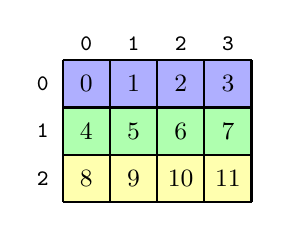
\begin{tikzpicture}[x={(0cm,-0.6cm)},y={(0.6cm,0cm)},every node/.style={minimum size=0.6cm, outer sep=0pt, font=\small}]
\node[fill={rgb,255:red,175;green,175;blue,255}] at (0,0) {0};
\node[fill={rgb,255:red,175;green,175;blue,255}] at (0,1) {1};
\node[fill={rgb,255:red,175;green,175;blue,255}] at (0,2) {2};
\node[fill={rgb,255:red,175;green,175;blue,255}] at (0,3) {3};
\node[fill={rgb,255:red,175;green,255;blue,175}] at (1,0) {4};
\node[fill={rgb,255:red,175;green,255;blue,175}] at (1,1) {5};
\node[fill={rgb,255:red,175;green,255;blue,175}] at (1,2) {6};
\node[fill={rgb,255:red,175;green,255;blue,175}] at (1,3) {7};
\node[fill={rgb,255:red,255;green,255;blue,175}] at (2,0) {8};
\node[fill={rgb,255:red,255;green,255;blue,175}] at (2,1) {9};
\node[fill={rgb,255:red,255;green,255;blue,175}] at (2,2) {10};
\node[fill={rgb,255:red,255;green,255;blue,175}] at (2,3) {11};
\draw[color=black,thick,step=0.6cm,shift={(-0.5,-0.5)}] (0,0) grid (3,4);
\node[anchor=east,minimum size=0pt,font=\footnotesize] at (0,-0.6) {\texttt{0}};
\node[anchor=east,minimum size=0pt,font=\footnotesize] at (1,-0.6) {\texttt{1}};
\node[anchor=east,minimum size=0pt,font=\footnotesize] at (2,-0.6) {\texttt{2}};
\node[minimum size=0pt,font=\footnotesize] at (-0.85,0) {\texttt{0}};
\node[minimum size=0pt,font=\footnotesize] at (-0.85,1) {\texttt{1}};
\node[minimum size=0pt,font=\footnotesize] at (-0.85,2) {\texttt{2}};
\node[minimum size=0pt,font=\footnotesize] at (-0.85,3) {\texttt{3}};
\end{tikzpicture}
\end{minipage}
\end{center}



\item[$\mathrm{split}(n{:}d,\, S)$] for $\size S = n$, the shape $S$ carrying
the strides of $\mathrm{canonical}(S)$ each multiplied by $d$, which for a flat
$S = (m_1,\dots,m_r)$ is
\[
(m_1,\dots,m_r) \;{:}\;
\Big(d\textstyle\prod_{i>1} m_i,\; d\prod_{i>2} m_i,\; \dots,\; d\,m_r,\; d\Big)
\]
and for a nested $S$ follows its nesting. The argument $n{:}\bot$ gives $S$
with every stride $\bot$.
\par\smallskip
\begin{center}
\begin{minipage}[t]{0.5\linewidth}\centering
$6{:}2$\\[4pt]
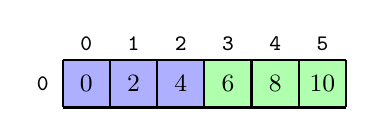
\begin{tikzpicture}[x={(0cm,-0.6cm)},y={(0.6cm,0cm)},every node/.style={minimum size=0.6cm, outer sep=0pt, font=\small}]
\node[fill={rgb,255:red,175;green,175;blue,255}] at (0,0) {0};
\node[fill={rgb,255:red,175;green,175;blue,255}] at (0,1) {2};
\node[fill={rgb,255:red,175;green,175;blue,255}] at (0,2) {4};
\node[fill={rgb,255:red,175;green,255;blue,175}] at (0,3) {6};
\node[fill={rgb,255:red,175;green,255;blue,175}] at (0,4) {8};
\node[fill={rgb,255:red,175;green,255;blue,175}] at (0,5) {10};
\draw[color=black,thick,step=0.6cm,shift={(-0.5,-0.5)}] (0,0) grid (1,6);
\node[anchor=east,minimum size=0pt,font=\footnotesize] at (0,-0.6) {\texttt{0}};
\node[minimum size=0pt,font=\footnotesize] at (-0.85,0) {\texttt{0}};
\node[minimum size=0pt,font=\footnotesize] at (-0.85,1) {\texttt{1}};
\node[minimum size=0pt,font=\footnotesize] at (-0.85,2) {\texttt{2}};
\node[minimum size=0pt,font=\footnotesize] at (-0.85,3) {\texttt{3}};
\node[minimum size=0pt,font=\footnotesize] at (-0.85,4) {\texttt{4}};
\node[minimum size=0pt,font=\footnotesize] at (-0.85,5) {\texttt{5}};
\end{tikzpicture}
\end{minipage}\hfill
\begin{minipage}[t]{0.45\linewidth}\centering
$\mathrm{split}(6{:}2,\,(2,3)) = (2,3){:}(6,2)$\\[4pt]
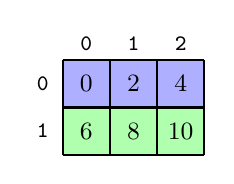
\begin{tikzpicture}[x={(0cm,-0.6cm)},y={(0.6cm,0cm)},every node/.style={minimum size=0.6cm, outer sep=0pt, font=\small}]
\node[fill={rgb,255:red,175;green,175;blue,255}] at (0,0) {0};
\node[fill={rgb,255:red,175;green,175;blue,255}] at (0,1) {2};
\node[fill={rgb,255:red,175;green,175;blue,255}] at (0,2) {4};
\node[fill={rgb,255:red,175;green,255;blue,175}] at (1,0) {6};
\node[fill={rgb,255:red,175;green,255;blue,175}] at (1,1) {8};
\node[fill={rgb,255:red,175;green,255;blue,175}] at (1,2) {10};
\draw[color=black,thick,step=0.6cm,shift={(-0.5,-0.5)}] (0,0) grid (2,3);
\node[anchor=east,minimum size=0pt,font=\footnotesize] at (0,-0.6) {\texttt{0}};
\node[anchor=east,minimum size=0pt,font=\footnotesize] at (1,-0.6) {\texttt{1}};
\node[minimum size=0pt,font=\footnotesize] at (-0.85,0) {\texttt{0}};
\node[minimum size=0pt,font=\footnotesize] at (-0.85,1) {\texttt{1}};
\node[minimum size=0pt,font=\footnotesize] at (-0.85,2) {\texttt{2}};
\end{tikzpicture}
\end{minipage}
\end{center}



\item[$\divideop(L, S)$] partitions $L$ into tiles of shape $S$. Let
$L = (n_1,\dots,n_m){:}(d_1,\dots,d_m)$ and let $S = (k_1,\dots,k_m)$ with
$k_i \mid n_i$. Each mode splits as
\[
\mathrm{split}\big(n_i{:}d_i,\; (n_i/k_i,\, k_i)\big)
\;=\; (n_i/k_i,\, k_i) \;{:}\; (k_i d_i,\, d_i),
\]
and collecting the second component of every split into one group and the
first into another gives
\[
\divideop(L,S) \;=\;
\big((k_1,\dots,k_m),\ (n_1/k_1,\dots,n_m/k_m)\big)
\;{:}\;
\big((d_1,\dots,d_m),\ (k_1d_1,\dots,k_md_m)\big).
\]
The first group indexes a mode inside a tile and the second indexes which
tile. It is easy to see that precomposing with the flattening that sends each pair
$(b_i, t_i)$ back to $c_i = b_i k_i + t_i$ recovers $L$.
\par\smallskip
\begin{center}
\begin{minipage}[t]{0.48\linewidth}\centering
$L = (4,6){:}(6,1)$, coloured by tile\\[4pt]
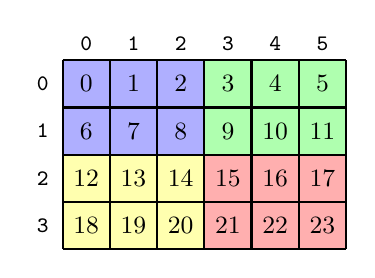
\begin{tikzpicture}[x={(0cm,-0.6cm)},y={(0.6cm,0cm)},every node/.style={minimum size=0.6cm, outer sep=0pt, font=\small}]
\node[fill={rgb,255:red,175;green,175;blue,255}] at (0,0) {0};
\node[fill={rgb,255:red,175;green,175;blue,255}] at (0,1) {1};
\node[fill={rgb,255:red,175;green,175;blue,255}] at (0,2) {2};
\node[fill={rgb,255:red,175;green,255;blue,175}] at (0,3) {3};
\node[fill={rgb,255:red,175;green,255;blue,175}] at (0,4) {4};
\node[fill={rgb,255:red,175;green,255;blue,175}] at (0,5) {5};
\node[fill={rgb,255:red,175;green,175;blue,255}] at (1,0) {6};
\node[fill={rgb,255:red,175;green,175;blue,255}] at (1,1) {7};
\node[fill={rgb,255:red,175;green,175;blue,255}] at (1,2) {8};
\node[fill={rgb,255:red,175;green,255;blue,175}] at (1,3) {9};
\node[fill={rgb,255:red,175;green,255;blue,175}] at (1,4) {10};
\node[fill={rgb,255:red,175;green,255;blue,175}] at (1,5) {11};
\node[fill={rgb,255:red,255;green,255;blue,175}] at (2,0) {12};
\node[fill={rgb,255:red,255;green,255;blue,175}] at (2,1) {13};
\node[fill={rgb,255:red,255;green,255;blue,175}] at (2,2) {14};
\node[fill={rgb,255:red,255;green,175;blue,175}] at (2,3) {15};
\node[fill={rgb,255:red,255;green,175;blue,175}] at (2,4) {16};
\node[fill={rgb,255:red,255;green,175;blue,175}] at (2,5) {17};
\node[fill={rgb,255:red,255;green,255;blue,175}] at (3,0) {18};
\node[fill={rgb,255:red,255;green,255;blue,175}] at (3,1) {19};
\node[fill={rgb,255:red,255;green,255;blue,175}] at (3,2) {20};
\node[fill={rgb,255:red,255;green,175;blue,175}] at (3,3) {21};
\node[fill={rgb,255:red,255;green,175;blue,175}] at (3,4) {22};
\node[fill={rgb,255:red,255;green,175;blue,175}] at (3,5) {23};
\draw[color=black,thick,step=0.6cm,shift={(-0.5,-0.5)}] (0,0) grid (4,6);
\node[anchor=east,minimum size=0pt,font=\footnotesize] at (0,-0.6) {\texttt{0}};
\node[anchor=east,minimum size=0pt,font=\footnotesize] at (1,-0.6) {\texttt{1}};
\node[anchor=east,minimum size=0pt,font=\footnotesize] at (2,-0.6) {\texttt{2}};
\node[anchor=east,minimum size=0pt,font=\footnotesize] at (3,-0.6) {\texttt{3}};
\node[minimum size=0pt,font=\footnotesize] at (-0.85,0) {\texttt{0}};
\node[minimum size=0pt,font=\footnotesize] at (-0.85,1) {\texttt{1}};
\node[minimum size=0pt,font=\footnotesize] at (-0.85,2) {\texttt{2}};
\node[minimum size=0pt,font=\footnotesize] at (-0.85,3) {\texttt{3}};
\node[minimum size=0pt,font=\footnotesize] at (-0.85,4) {\texttt{4}};
\node[minimum size=0pt,font=\footnotesize] at (-0.85,5) {\texttt{5}};
\end{tikzpicture}
\end{minipage}\hfill
\begin{minipage}[t]{0.48\linewidth}\centering
$\divideop(L,(2,3))$: tile coordinate $(t_1,t_2)$ as row, tile $(b_1,b_2)$ as column\\[4pt]
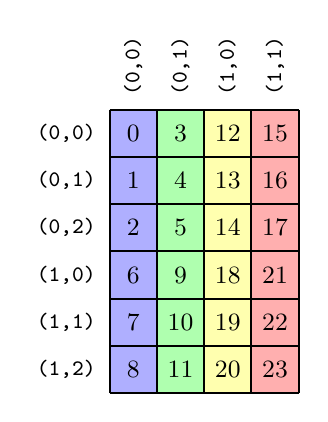
\begin{tikzpicture}[x={(0cm,-0.6cm)},y={(0.6cm,0cm)},every node/.style={minimum size=0.6cm, outer sep=0pt, font=\small}]
\node[fill={rgb,255:red,175;green,175;blue,255}] at (0,0) {0};
\node[fill={rgb,255:red,175;green,255;blue,175}] at (0,1) {3};
\node[fill={rgb,255:red,255;green,255;blue,175}] at (0,2) {12};
\node[fill={rgb,255:red,255;green,175;blue,175}] at (0,3) {15};
\node[fill={rgb,255:red,175;green,175;blue,255}] at (1,0) {1};
\node[fill={rgb,255:red,175;green,255;blue,175}] at (1,1) {4};
\node[fill={rgb,255:red,255;green,255;blue,175}] at (1,2) {13};
\node[fill={rgb,255:red,255;green,175;blue,175}] at (1,3) {16};
\node[fill={rgb,255:red,175;green,175;blue,255}] at (2,0) {2};
\node[fill={rgb,255:red,175;green,255;blue,175}] at (2,1) {5};
\node[fill={rgb,255:red,255;green,255;blue,175}] at (2,2) {14};
\node[fill={rgb,255:red,255;green,175;blue,175}] at (2,3) {17};
\node[fill={rgb,255:red,175;green,175;blue,255}] at (3,0) {6};
\node[fill={rgb,255:red,175;green,255;blue,175}] at (3,1) {9};
\node[fill={rgb,255:red,255;green,255;blue,175}] at (3,2) {18};
\node[fill={rgb,255:red,255;green,175;blue,175}] at (3,3) {21};
\node[fill={rgb,255:red,175;green,175;blue,255}] at (4,0) {7};
\node[fill={rgb,255:red,175;green,255;blue,175}] at (4,1) {10};
\node[fill={rgb,255:red,255;green,255;blue,175}] at (4,2) {19};
\node[fill={rgb,255:red,255;green,175;blue,175}] at (4,3) {22};
\node[fill={rgb,255:red,175;green,175;blue,255}] at (5,0) {8};
\node[fill={rgb,255:red,175;green,255;blue,175}] at (5,1) {11};
\node[fill={rgb,255:red,255;green,255;blue,175}] at (5,2) {20};
\node[fill={rgb,255:red,255;green,175;blue,175}] at (5,3) {23};
\draw[color=black,thick,step=0.6cm,shift={(-0.5,-0.5)}] (0,0) grid (6,4);
\node[anchor=east,minimum size=0pt,font=\footnotesize] at (0,-0.6) {\texttt{(0,0)}};
\node[anchor=east,minimum size=0pt,font=\footnotesize] at (1,-0.6) {\texttt{(0,1)}};
\node[anchor=east,minimum size=0pt,font=\footnotesize] at (2,-0.6) {\texttt{(0,2)}};
\node[anchor=east,minimum size=0pt,font=\footnotesize] at (3,-0.6) {\texttt{(1,0)}};
\node[anchor=east,minimum size=0pt,font=\footnotesize] at (4,-0.6) {\texttt{(1,1)}};
\node[anchor=east,minimum size=0pt,font=\footnotesize] at (5,-0.6) {\texttt{(1,2)}};
\node[rotate=90,anchor=west,minimum size=0pt,font=\footnotesize] at (-0.6,0) {\texttt{(0,0)}};
\node[rotate=90,anchor=west,minimum size=0pt,font=\footnotesize] at (-0.6,1) {\texttt{(0,1)}};
\node[rotate=90,anchor=west,minimum size=0pt,font=\footnotesize] at (-0.6,2) {\texttt{(1,0)}};
\node[rotate=90,anchor=west,minimum size=0pt,font=\footnotesize] at (-0.6,3) {\texttt{(1,1)}};
\end{tikzpicture}
\end{minipage}
\end{center}



\item[$\repeatop(L, A)$] copies of $L$ arranged in the layout of $A$, which is
required to be a valid $\logical \to \logical$ layout and so a dense bijection:
\[
\repeatop(L,A) \;=\; (S_A, S_L) \;{:}\; \big((\cosize L)\,D_A,\ D_L\big),
\]
where $L = S_L{:}D_L$, $A = S_A{:}D_A$, and $c\,D$ multiplies every stride of
$D$ by $c$.
If $L$ is a dense bijection then $\cosize L = \size L$, and the addresses
$(\size L)\,A(a) + L(v)$ take every value in $[0, \size A \cdot \size L)$
exactly once: the result is a dense bijection.

When $L$ carries a swizzle $\sigma$, $\repeatop$ is defined only if $\cosize L$
is a power of two, $2^p$, and both fields of $\sigma$ lie below bit $p$. Then
$\sigma\big((\cosize L)\,a + x\big) = (\cosize L)\,a + \sigma(x)$ and every
copy is swizzled alike. Otherwise the copy index reaches the bits $\sigma$
reads, and the operation rejects.

\item[$\interleave(L, A)$] the same copies interleaved element by element
rather than laid out one after another, with $A$ again a valid
$\logical \to \logical$ layout:
\[
\interleave(L,A) \;=\; (S_A, S_L) \;{:}\; \big(D_A,\ (\size A)\,D_L\big).
\]
The coordinate $(a,v)$ lands at $A(a) + (\size A)\,L(v)$, so each element of
$L$ becomes a run of $\size A$ consecutive addresses holding that element of
every copy, where $\repeatop$ instead gives each copy a run of its own. If $L$
is a dense bijection the result is again a dense bijection onto
$[0, \size A \cdot \size L)$. On a swizzled $L$ it has no defined meaning
and rejects.
\par\smallskip
\begin{center}
\begin{minipage}[t]{0.2\linewidth}\centering
$L = (2,2){:}(2,1)$\\[4pt]
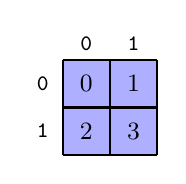
\begin{tikzpicture}[x={(0cm,-0.6cm)},y={(0.6cm,0cm)},every node/.style={minimum size=0.6cm, outer sep=0pt, font=\small}]
\node[fill={rgb,255:red,175;green,175;blue,255}] at (0,0) {0};
\node[fill={rgb,255:red,175;green,175;blue,255}] at (0,1) {1};
\node[fill={rgb,255:red,175;green,175;blue,255}] at (1,0) {2};
\node[fill={rgb,255:red,175;green,175;blue,255}] at (1,1) {3};
\draw[color=black,thick,step=0.6cm,shift={(-0.5,-0.5)}] (0,0) grid (2,2);
\node[anchor=east,minimum size=0pt,font=\footnotesize] at (0,-0.6) {\texttt{0}};
\node[anchor=east,minimum size=0pt,font=\footnotesize] at (1,-0.6) {\texttt{1}};
\node[minimum size=0pt,font=\footnotesize] at (-0.85,0) {\texttt{0}};
\node[minimum size=0pt,font=\footnotesize] at (-0.85,1) {\texttt{1}};
\end{tikzpicture}
\end{minipage}\hfill
\begin{minipage}[t]{0.38\linewidth}\centering
$\repeatop(L,\,3{:}1) = (3,(2,2)){:}(4,(2,1))$\\[4pt]
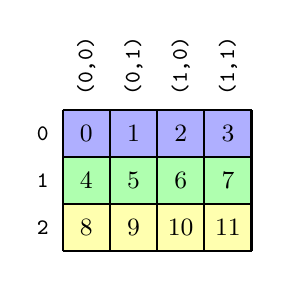
\begin{tikzpicture}[x={(0cm,-0.6cm)},y={(0.6cm,0cm)},every node/.style={minimum size=0.6cm, outer sep=0pt, font=\small}]
\node[fill={rgb,255:red,175;green,175;blue,255}] at (0,0) {0};
\node[fill={rgb,255:red,175;green,175;blue,255}] at (0,1) {1};
\node[fill={rgb,255:red,175;green,175;blue,255}] at (0,2) {2};
\node[fill={rgb,255:red,175;green,175;blue,255}] at (0,3) {3};
\node[fill={rgb,255:red,175;green,255;blue,175}] at (1,0) {4};
\node[fill={rgb,255:red,175;green,255;blue,175}] at (1,1) {5};
\node[fill={rgb,255:red,175;green,255;blue,175}] at (1,2) {6};
\node[fill={rgb,255:red,175;green,255;blue,175}] at (1,3) {7};
\node[fill={rgb,255:red,255;green,255;blue,175}] at (2,0) {8};
\node[fill={rgb,255:red,255;green,255;blue,175}] at (2,1) {9};
\node[fill={rgb,255:red,255;green,255;blue,175}] at (2,2) {10};
\node[fill={rgb,255:red,255;green,255;blue,175}] at (2,3) {11};
\draw[color=black,thick,step=0.6cm,shift={(-0.5,-0.5)}] (0,0) grid (3,4);
\node[anchor=east,minimum size=0pt,font=\footnotesize] at (0,-0.6) {\texttt{0}};
\node[anchor=east,minimum size=0pt,font=\footnotesize] at (1,-0.6) {\texttt{1}};
\node[anchor=east,minimum size=0pt,font=\footnotesize] at (2,-0.6) {\texttt{2}};
\node[rotate=90,anchor=west,minimum size=0pt,font=\footnotesize] at (-0.6,0) {\texttt{(0,0)}};
\node[rotate=90,anchor=west,minimum size=0pt,font=\footnotesize] at (-0.6,1) {\texttt{(0,1)}};
\node[rotate=90,anchor=west,minimum size=0pt,font=\footnotesize] at (-0.6,2) {\texttt{(1,0)}};
\node[rotate=90,anchor=west,minimum size=0pt,font=\footnotesize] at (-0.6,3) {\texttt{(1,1)}};
\end{tikzpicture}
\end{minipage}\hfill
\begin{minipage}[t]{0.38\linewidth}\centering
$\interleave(L,\,3{:}1) = (3,(2,2)){:}(1,(6,3))$\\[4pt]
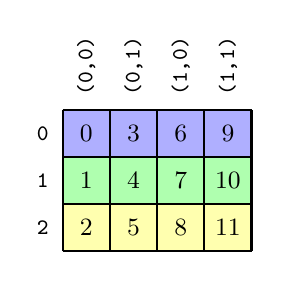
\begin{tikzpicture}[x={(0cm,-0.6cm)},y={(0.6cm,0cm)},every node/.style={minimum size=0.6cm, outer sep=0pt, font=\small}]
\node[fill={rgb,255:red,175;green,175;blue,255}] at (0,0) {0};
\node[fill={rgb,255:red,175;green,175;blue,255}] at (0,1) {3};
\node[fill={rgb,255:red,175;green,175;blue,255}] at (0,2) {6};
\node[fill={rgb,255:red,175;green,175;blue,255}] at (0,3) {9};
\node[fill={rgb,255:red,175;green,255;blue,175}] at (1,0) {1};
\node[fill={rgb,255:red,175;green,255;blue,175}] at (1,1) {4};
\node[fill={rgb,255:red,175;green,255;blue,175}] at (1,2) {7};
\node[fill={rgb,255:red,175;green,255;blue,175}] at (1,3) {10};
\node[fill={rgb,255:red,255;green,255;blue,175}] at (2,0) {2};
\node[fill={rgb,255:red,255;green,255;blue,175}] at (2,1) {5};
\node[fill={rgb,255:red,255;green,255;blue,175}] at (2,2) {8};
\node[fill={rgb,255:red,255;green,255;blue,175}] at (2,3) {11};
\draw[color=black,thick,step=0.6cm,shift={(-0.5,-0.5)}] (0,0) grid (3,4);
\node[anchor=east,minimum size=0pt,font=\footnotesize] at (0,-0.6) {\texttt{0}};
\node[anchor=east,minimum size=0pt,font=\footnotesize] at (1,-0.6) {\texttt{1}};
\node[anchor=east,minimum size=0pt,font=\footnotesize] at (2,-0.6) {\texttt{2}};
\node[rotate=90,anchor=west,minimum size=0pt,font=\footnotesize] at (-0.6,0) {\texttt{(0,0)}};
\node[rotate=90,anchor=west,minimum size=0pt,font=\footnotesize] at (-0.6,1) {\texttt{(0,1)}};
\node[rotate=90,anchor=west,minimum size=0pt,font=\footnotesize] at (-0.6,2) {\texttt{(1,0)}};
\node[rotate=90,anchor=west,minimum size=0pt,font=\footnotesize] at (-0.6,3) {\texttt{(1,1)}};
\end{tikzpicture}
\end{minipage}
\end{center}



\item[$\broadcast(L, S)$] $\size S$ copies of $L$ at the same addresses:
\[
\broadcast(L,S) \;=\; (S, S_L) \;{:}\; (\bot,\ D_L),
\]
writing $\bot$ for the stride with $\bot$ at every entry of $S$. The coordinate
$(a,v)$ lands at $L(v)$ whatever $a$ is. The second argument is a shape and not
a layout because the copies share their addresses and so have no strides to
carry. The result is valid when $L$ is, and not write-valid once
$\size S \ge 2$.
\par\smallskip
\begin{center}
\begin{minipage}[t]{0.6\linewidth}\centering
$\broadcast(4{:}1,\,(3)) = (3,4){:}(\bot,1)$: copy as row\\[4pt]
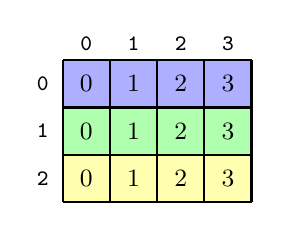
\begin{tikzpicture}[x={(0cm,-0.6cm)},y={(0.6cm,0cm)},every node/.style={minimum size=0.6cm, outer sep=0pt, font=\small}]
\node[fill={rgb,255:red,175;green,175;blue,255}] at (0,0) {0};
\node[fill={rgb,255:red,175;green,175;blue,255}] at (0,1) {1};
\node[fill={rgb,255:red,175;green,175;blue,255}] at (0,2) {2};
\node[fill={rgb,255:red,175;green,175;blue,255}] at (0,3) {3};
\node[fill={rgb,255:red,175;green,255;blue,175}] at (1,0) {0};
\node[fill={rgb,255:red,175;green,255;blue,175}] at (1,1) {1};
\node[fill={rgb,255:red,175;green,255;blue,175}] at (1,2) {2};
\node[fill={rgb,255:red,175;green,255;blue,175}] at (1,3) {3};
\node[fill={rgb,255:red,255;green,255;blue,175}] at (2,0) {0};
\node[fill={rgb,255:red,255;green,255;blue,175}] at (2,1) {1};
\node[fill={rgb,255:red,255;green,255;blue,175}] at (2,2) {2};
\node[fill={rgb,255:red,255;green,255;blue,175}] at (2,3) {3};
\draw[color=black,thick,step=0.6cm,shift={(-0.5,-0.5)}] (0,0) grid (3,4);
\node[anchor=east,minimum size=0pt,font=\footnotesize] at (0,-0.6) {\texttt{0}};
\node[anchor=east,minimum size=0pt,font=\footnotesize] at (1,-0.6) {\texttt{1}};
\node[anchor=east,minimum size=0pt,font=\footnotesize] at (2,-0.6) {\texttt{2}};
\node[minimum size=0pt,font=\footnotesize] at (-0.85,0) {\texttt{0}};
\node[minimum size=0pt,font=\footnotesize] at (-0.85,1) {\texttt{1}};
\node[minimum size=0pt,font=\footnotesize] at (-0.85,2) {\texttt{2}};
\node[minimum size=0pt,font=\footnotesize] at (-0.85,3) {\texttt{3}};
\end{tikzpicture}
\end{minipage}
\end{center}



\item[$\mathrm{inverse}(L)$] for $L$ a flat dense bijection with modes
$(n_1,\dots,n_m){:}(d_1,\dots,d_m)$, every $n_i \ge 2$; as in
Lemma~\ref{lem:dense}, modes of size $1$ are dropped first. Give mode $i$ the canonical weight
$w_i = \prod_{j>i} n_j$ and list the modes in decreasing order of stride. Then
\[
\mathrm{inverse}(L) \;=\;
(n_{(1)},\dots,n_{(m)}) \;{:}\; (w_{(1)},\dots,w_{(m)}),
\]
again a dense bijection. Read both as maps on $[0,N)$, each unflattening the
integer it is given into its own shape, and they are mutually inverse.
\par\smallskip
\begin{center}
\begin{minipage}[t]{0.45\linewidth}\centering
$L = (2,3){:}(1,2)$, coloured by element\\[4pt]
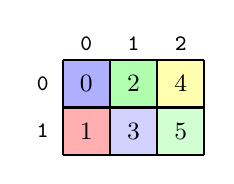
\begin{tikzpicture}[x={(0cm,-0.6cm)},y={(0.6cm,0cm)},every node/.style={minimum size=0.6cm, outer sep=0pt, font=\small}]
\node[fill={rgb,255:red,175;green,175;blue,255}] at (0,0) {0};
\node[fill={rgb,255:red,175;green,255;blue,175}] at (0,1) {2};
\node[fill={rgb,255:red,255;green,255;blue,175}] at (0,2) {4};
\node[fill={rgb,255:red,255;green,175;blue,175}] at (1,0) {1};
\node[fill={rgb,255:red,210;green,210;blue,255}] at (1,1) {3};
\node[fill={rgb,255:red,210;green,255;blue,210}] at (1,2) {5};
\draw[color=black,thick,step=0.6cm,shift={(-0.5,-0.5)}] (0,0) grid (2,3);
\node[anchor=east,minimum size=0pt,font=\footnotesize] at (0,-0.6) {\texttt{0}};
\node[anchor=east,minimum size=0pt,font=\footnotesize] at (1,-0.6) {\texttt{1}};
\node[minimum size=0pt,font=\footnotesize] at (-0.85,0) {\texttt{0}};
\node[minimum size=0pt,font=\footnotesize] at (-0.85,1) {\texttt{1}};
\node[minimum size=0pt,font=\footnotesize] at (-0.85,2) {\texttt{2}};
\end{tikzpicture}
\end{minipage}\hfill
\begin{minipage}[t]{0.5\linewidth}\centering
$\mathrm{inverse}(L) = (3,2){:}(1,3)$, at address $2a+b$ the element $a+3b$\\[4pt]
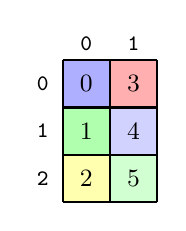
\begin{tikzpicture}[x={(0cm,-0.6cm)},y={(0.6cm,0cm)},every node/.style={minimum size=0.6cm, outer sep=0pt, font=\small}]
\node[fill={rgb,255:red,175;green,175;blue,255}] at (0,0) {0};
\node[fill={rgb,255:red,255;green,175;blue,175}] at (0,1) {3};
\node[fill={rgb,255:red,175;green,255;blue,175}] at (1,0) {1};
\node[fill={rgb,255:red,210;green,210;blue,255}] at (1,1) {4};
\node[fill={rgb,255:red,255;green,255;blue,175}] at (2,0) {2};
\node[fill={rgb,255:red,210;green,255;blue,210}] at (2,1) {5};
\draw[color=black,thick,step=0.6cm,shift={(-0.5,-0.5)}] (0,0) grid (3,2);
\node[anchor=east,minimum size=0pt,font=\footnotesize] at (0,-0.6) {\texttt{0}};
\node[anchor=east,minimum size=0pt,font=\footnotesize] at (1,-0.6) {\texttt{1}};
\node[anchor=east,minimum size=0pt,font=\footnotesize] at (2,-0.6) {\texttt{2}};
\node[minimum size=0pt,font=\footnotesize] at (-0.85,0) {\texttt{0}};
\node[minimum size=0pt,font=\footnotesize] at (-0.85,1) {\texttt{1}};
\end{tikzpicture}
\end{minipage}
\end{center}


\end{description}

\section{Deciding whether a composite is a layout}\label{sec:decide}

While a composite can be natively emitted as is, sometimes we can simplify the codegen
if that composite is actually itself a layout.

Fix a map $f : \mathrm{Coord}(S) \to \Z$ on a shape $S = (n_1,\dots,n_m)$.
We take $S$ flat, since a nested shape has the coordinates of the flat shape
of its leaves, regrouped. Write $c = (c_1,\dots,c_m)$ for a coordinate and
$\mathbf{0}$ for the origin. Every layout sends $\mathbf{0}$ to $0$, and
composition and swizzle preserve this, so $f(\mathbf{0}) = 0$ for every
composite. Maps take values in $\Z$ throughout this section: strides are
integers, and Section~\ref{sec:restrict} subtracts a constant.

\begin{definition}[Refinement]\label{def:refine}
A \emph{refinement} of a flat shape $S = (n_1,\dots,n_m)$ is a shape
$S' = (S_1,\dots,S_m)$ with each $S_i$ flat and $\size S_i = n_i$. A
coordinate of $S_i$ is identified with its flattening in $[0,n_i)$
(Definition~\ref{def:layout}), so $\mathrm{Coord}(S')$ and $\mathrm{Coord}(S)$
are the same set. A map $f : \mathrm{Coord}(S) \to \Z$ \emph{is the layout}
$S'{:}D'$ when
\[
f(c_1,\dots,c_m) \;=\;
(S'{:}D')\big(\mathrm{unflatten}_{S_1}(c_1),\,\dots,\,\mathrm{unflatten}_{S_m}(c_m)\big)
\]
for every coordinate; for $S' = S$ this says $f = S{:}D$. The question of
this section is whether $f$ is a layout $S'{:}D'$ for some refinement $S'$ of
$S$ and some stride $D'$.
\end{definition}

\begin{lemma}[Separability]\label{lem:separable}
Let $S = (n_1,\dots,n_m)$ be a flat shape and $f : \mathrm{Coord}(S) \to \Z$.
For $1 \le i \le m$ let $e_i$ be the coordinate with entry $i$ equal to $1$
and every other entry $0$, and define $g_i : [0,n_i) \to \Z$ by
$g_i(v) = f(v\,e_i)$. Then $f$ is a layout $S'{:}D'$ for some refinement $S'$
of $S$ if and only if
\begin{equation}\label{eq:sep}
f(c) = \sum_{i=1}^{m} g_i(c_i)
\quad\text{for every } c = (c_1,\dots,c_m) \in \mathrm{Coord}(S),
\end{equation}
and each $g_i$ is a layout of some flat shape of size $n_i$.
\end{lemma}
\begin{proof}
($\Rightarrow$) Let $f = S'{:}(D_1,\dots,D_m)$ with $S' = (S_1,\dots,S_m)$.
By Definition~\ref{def:layout},
\[
f(c) = \sum_{i=1}^{m} (S_i{:}D_i)\big(\mathrm{unflatten}_{S_i}(c_i)\big)
\quad\text{for every } c.
\]
At $c = v\,e_i$ every term but the $i$th is a layout evaluated at coordinate
$0$, hence $0$, so $g_i(v) = (S_i{:}D_i)(\mathrm{unflatten}_{S_i}(v))$: the
$i$th term is $g_i(c_i)$, which is \eqref{eq:sep}, and $g_i = S_i{:}D_i$.
($\Leftarrow$) If $g_i = S_i{:}D_i$ for each $i$, the same identity read
backwards gives $f = (S_1,\dots,S_m){:}(D_1,\dots,D_m)$.
\end{proof}

Checking \eqref{eq:sep} is one pass over $\mathrm{Coord}(S)$. What remains
is one coordinate at a time: a map $g : [0,n) \to \Z$ with $g(0) = 0$, and
the question whether there is a flat shape $T$ of size $n$ and a stride $D$
with $g = (T{:}D) \circ \mathrm{unflatten}_T$. To decide it we need this
composite as a formula in $v$.

Number the entries of $T$ from the right, $T = (m_k,\dots,m_1)$, so that
indices increase with the weights $w_j$ below. By Definition~\ref{def:layout},
$\mathrm{unflatten}_T(v)$ is the coordinate $(x_k,\dots,x_1)$ of $T$ with
\[
v = \sum_{j=1}^{k} x_j\, w_j, \qquad w_j = m_1 m_2 \cdots m_{j-1},
\]
the $w_j$ being the strides of $\mathrm{canonical}(T)$; so $w_1 = 1$,
$w_{j+1} = w_j m_j$, and $w_k m_k = n$. Solving for the components,
\[
x_j = \lfloor v / w_j \rfloor \bmod m_j,
\]
which we write $d_j(v)$. Therefore
\[
\big(T{:}(s_k,\dots,s_1)\big)\big(\mathrm{unflatten}_T(v)\big)
\;=\; \sum_{j=1}^{k} s_j\, d_j(v),
\]
and $g$ is the layout $T{:}(s_k,\dots,s_1)$ exactly when $g(v)$ equals this
sum for every $v \in [0,n)$.

Two remarks turn the search for $T$ into a search for the $w_j$. An entry
with $m_j = 1$ has $d_j = 0$ and contributes nothing, so we assume $T$ has
none; then $1 = w_1 < w_2 < \cdots < w_k < n$, each dividing the next and
$w_k$ dividing $n$, which we write $1 = w_1 \mid w_2 \mid \cdots \mid w_k
\mid n$ and call the \emph{chain} of $T$. Conversely, every such chain is
the chain of exactly one such $T$, given by $m_j = w_{j+1}/w_j$ with
$w_{k+1} = n$. Theorem~\ref{thm:decide} finds $T$ by finding its chain.

Each component $d_j(v) = \lfloor v/w_j \rfloor \bmod m_j$ is the remainder
of $\lfloor v/w_j \rfloor$ on division by $m_j$. The lemma rewrites
$\sum_j s_j\, d_j(v)$ with floors alone.

\begin{lemma}[Components as differences of floors]\label{lem:floor}
For positive integers $w \mid w'$ and every integer $v \ge 0$,
\[
\lfloor v/w \rfloor \bmod (w'/w) \;=\;
\lfloor v/w \rfloor - (w'/w)\lfloor v/w' \rfloor .
\]
Let $T$ be a flat shape of size $n$ with $k$ entries, with chain
$1 = w_1 \mid \cdots \mid w_k \mid n$, entry sizes $m_j$, and components
$d_j$ as above, and let integers $s_1,\dots,s_k$ and $a_1,\dots,a_k$ be
related by
\[
a_j = s_j - m_{j-1}\,s_{j-1} \quad (1 \le j \le k), \qquad m_0 s_0 = 0,
\]
a relation that determines either family from the other. Then for a map
$g : [0,n) \to \Z$,
\[
g(v) = \sum_{j=1}^{k} s_j\, d_j(v) \ \text{ for every } v \in [0,n)
\quad\Longleftrightarrow\quad
g(v) = \sum_{j=1}^{k} a_j \lfloor v/w_j \rfloor \ \text{ for every } v \in [0,n),
\]
and when these hold, $s_j = g(w_j)$.
\end{lemma}
\begin{proof}
Write $q = \lfloor v/w \rfloor$ and $r = w'/w$. The remainder of $q$ on
division by $r$ is $q - r\lfloor q/r \rfloor$, and $\lfloor q/r \rfloor =
\lfloor v/(wr) \rfloor = \lfloor v/w' \rfloor$ for positive integers $w, r$,
which is the identity. With $w = w_j$, $w' = w_{j+1}$, and $w'/w = m_j$ it
reads
\[
d_j(v) = \lfloor v/w_j \rfloor - m_j \lfloor v/w_{j+1} \rfloor,
\]
where for $j = k$, $\lfloor v/w_{k+1} \rfloor = \lfloor v/n \rfloor = 0$ on
$[0,n)$. Hence
\[
\sum_{j=1}^{k} s_j\, d_j(v)
= \sum_{j=1}^{k} s_j \lfloor v/w_j \rfloor
  - \sum_{j=1}^{k-1} s_j m_j \lfloor v/w_{j+1} \rfloor
= \sum_{j=1}^{k} \big(s_j - m_{j-1}s_{j-1}\big) \lfloor v/w_j \rfloor
= \sum_{j=1}^{k} a_j \lfloor v/w_j \rfloor ,
\]
which is the equivalence. The relation gives $s_j = a_j + m_{j-1}s_{j-1}$,
so either family determines the other. Finally,
$d_l(w_j) = \lfloor w_j/w_l \rfloor \bmod m_l$ is $0$ for $l > j$ because
$w_j < w_l$, is $1$ for $l = j$ because $m_j \ge 2$, and is $0$ for $l < j$
because $w_j/w_l$ is a multiple of $w_{l+1}/w_l = m_l$; so
$g(w_j) = \sum_l s_l\, d_l(w_j) = s_j$.
\end{proof}

With floors alone, first differences read the chain off $g$, because
$\lfloor t/w \rfloor - \lfloor (t-1)/w \rfloor$ is $1$ if $w \mid t$ and $0$
otherwise.

\begin{theorem}[Linear recognition]\label{thm:decide}
Let $n \ge 2$ (for $n = 1$, $g = 0$ is the layout $(1){:}0$), let
$g : [0,n) \to \Z$ with $g(0) = 0$, and let $h(t) = g(t) - g(t-1)$ for
$1 \le t < n$. Run the following scan. Keep a copy $\rho$ of $h$, an integer
$w_{\mathrm{last}}$ initially $1$, and a set $R$ initially empty. For
$t = 1, 2, \dots, n-1$ in order, if $\rho(t) \ne 0$: if $t \nmid n$ or
$w_{\mathrm{last}} \nmid t$, reject; otherwise put $t$ in $R$, set
$a_t = \rho(t)$ and $w_{\mathrm{last}} = t$, and replace $\rho(t')$ by
$\rho(t') - a_t$ for every multiple $t'$ of $t$ in $[t, n)$. If no $t$
rejects, accept.

Then $g$ is a layout of some flat shape of size $n$ if and only if the scan
accepts. If it accepts, $\{1\} \cup R$ is the chain of a flat shape $T$ of
size $n$; $g$ is the layout $T{:}(s_k,\dots,s_1)$ with $s_j = g(w_j)$; and
every flat shape of size $n$ without entries of size $1$ of which $g$ is a
layout has a chain containing $\{1\} \cup R$. We call this $T$ the
\emph{coarsest}. The scan takes $O(n)$ arithmetic operations.
\end{theorem}
\begin{proof}
By Lemma~\ref{lem:floor}, $g$ is a layout of the shape with chain $W$ if
and only if there are integers $a_w$, $w \in W$, with
$g(v) = \sum_{w \in W} a_w \lfloor v/w \rfloor$ for every $v \in [0,n)$.
Since $\lfloor t/w \rfloor - \lfloor (t-1)/w \rfloor = [\,w \mid t\,]$ and
$g(0) = 0 = \sum_{w} a_w \lfloor 0/w \rfloor$, this is equivalent to
\begin{equation}\label{eq:diff}
h(t) = \sum_{w \in W} a_w\, [\,w \mid t\,] \quad\text{for } 1 \le t < n.
\end{equation}

Suppose \eqref{eq:diff} holds for some chain $W$ and coefficients $a_w$. We
show by induction on $t$ that when the scan reaches $t$,
$R = \{\, w \in W : w < t,\ a_w \ne 0 \,\}$ with the recorded $a_w$ equal
to those of \eqref{eq:diff}, and $\rho(t) = a_t$ if $t \in W$ and
$\rho(t) = 0$ otherwise. At $t = 1$, $R$ is empty and $\rho(1) = h(1) =
a_1$ because $1 \in W$ is the only divisor of $1$. Given the claim at $t$:
$\rho(t) = h(t) - \sum_{w \in R,\, w \mid t} a_w = \sum_{w \in W,\, w \mid t}
a_w - \sum_{w \in W,\, w < t,\, w \mid t} a_w = [\,t \in W\,]\, a_t$. If
$\rho(t) \ne 0$ then $t \in W$ and $a_t \ne 0$; $t \mid n$ because every
element of $W$ divides $n$; and $w_{\mathrm{last}}$, which is the largest
element of $R$ or else $1$, lies in $W$ below $t$ and so divides $t$
because $W$ is a chain. The scan records $t$ with $a_t$, and the claim
holds at $t+1$; if $\rho(t) = 0$ nothing is recorded and the claim holds at
$t+1$ as well. So the scan accepts, and $R \subseteq W$; with $1 \in W$,
$\{1\} \cup R \subseteq W$.

Conversely suppose the scan accepts. At each $t$ either $\rho(t)$ was $0$
or $a_t = \rho(t)$ was subtracted from it, and later steps change $\rho$
only at or beyond their own $t$; so at the end $\rho \equiv 0$, that is,
$h(t) = \sum_{w \in R,\, w \mid t} a_w$ for $1 \le t < n$. Every element of
$R$ divides $n$, lies below $n$, and is a multiple of the element recorded
before it or of $1$, so $\{1\} \cup R$ is a chain; let $T$ be its shape,
and put $a_1 = 0$ if $1 \notin R$. Then \eqref{eq:diff} holds for
$W = \{1\} \cup R$, so $g$ is a layout of $T$ by Lemma~\ref{lem:floor}, with
strides $s_j = g(w_j)$.

Each element of $R$ is at least twice the one before, so the subtractions
touch fewer than $n + n/2 + n/4 + \cdots < 2n$ entries of $\rho$; the rest
of the scan is one pass over $t$.
\end{proof}

The methodology is similar to Appendix~A.2.1 of Axe~\cite{axe}.

Codegen therefore emits one of two expressions. If the map is a layout
$S'{:}D'$ for a refinement $S' = (S_1,\dots,S_m)$, it emits
$\sum_{i,j} s_{ij}\, d_{ij}(c_i)$, with $d_{ij}$ the components of
$\mathrm{unflatten}_{S_i}(c_i)$, for the coarsest $S'$; no such expression has
fewer terms. Otherwise it emits the composite as Definition~\ref{def:compose}
writes it: the value of the right operand, unflattened into the left operand's
domain shape, evaluated by the left operand. Section~\ref{sec:restrict}
extends this to restricted maps, which do not vanish at the origin.

\section{Restriction}\label{sec:restrict}

A warp or a thread uses one slice of an address map: the map with its own
warp and thread coordinates fixed.

\begin{definition}[Restriction]\label{def:restrict}
Let $f : \mathrm{Coord}(S) \to \N$ with $S = (n_1,\dots,n_m)$ flat, let
$F \subseteq \{1,\dots,m\}$, and let $p_i \in [0,n_i)$ for each $i \in F$.
The \emph{restriction} of $f$ to $p$ is the map $f|_p$ on the coordinates of
the shape $(n_i)_{i \notin F}$ given by
\[
f|_p(c) = f(c'), \qquad
c'_i = \begin{cases} p_i & i \in F,\\ c_i & i \notin F. \end{cases}
\]
\end{definition}

$f|_p$ is in general not a layout: $f|_p(\mathbf{0})$ is the contribution
of the fixed entries, which need not be $0$, while every layout vanishes at
$\mathbf{0}$.

$f|_p$ is in general not dense, since its image omits the other slices, so
it is not a valid map into $\logical$ or $\tv$ (Definition~\ref{def:validity})
and cannot be the right operand of a composition
(Definition~\ref{def:compose}). Restriction is therefore allowed only for
maps into $\physical$, and is applied after composition, where the warp and
thread coordinates are entries of the composite's domain. Restricting a
restriction is restricting by the union of the fixed entries.

The address expression of a slice is Section~\ref{sec:decide} applied to
$f|_p - f|_p(\mathbf{0})$, which vanishes at the origin, plus the constant
$f|_p(\mathbf{0})$; when that map is not a layout, the composite's expression
is emitted with the fixed coordinates replaced by their values. The difference
can take negative values, which is why Section~\ref{sec:decide} is stated
over $\Z$: for $(2,2){:}(2,1)$ under the swizzle with $b = 1$, $\mathit{src} = 1$, $\mathit{dst} = 0$
(Definition~\ref{def:swizzle}), that is $\sigma(x) = x \oplus ((x \gg 1) \wedge 1)$,
$f(a,b) = (2a+b) \oplus a$, fixing $a = 1$ gives $f|_p(b) = 3 - b$ and
$f|_p - f|_p(\mathbf{0}) = -b$. The emitted arithmetic then carries a negative
coefficient. For
$f = (4,8,4){:}(32,1,8)$, $F = \{1\}$ and $p_1 = 2$, the slice is
$f|_p(r,v) = 64 + r + 8v$.

\section{CuTe in this algebra}\label{sec:cute}\label{sec:idioms}

CuTe lists the modes of a layout with the first varying fastest; we reverse
the list, recursively, and the two then agree as functions on the same
integers. CuTe's $\mathrm{composition}(A,B)$ applies $B$ first and is
$A \circ B$ in our algebra, with $B$ the right operand of
Definition~\ref{def:compose}. We take the four operations in the order of
Section~\ref{sec:intro}, state what each is in our algebra, and name the
documented examples~\cite{cutedocs} on which
the two are checked to agree.

\paragraph{Composition.} In CuTe, $\mathrm{composition}(A,B)$ is the layout
$L$ with $L(c) = A(B(c))$ for every $c \in \mathrm{Coord}(S_B)$. In our
algebra, $A \circ B$ is the map $c \mapsto A(\mathrm{unflatten}_{S_A}(B(c)))$, defined whenever $B$
is a dense bijection onto $[0,\size A)$, and Theorem~\ref{thm:decide} decides
whether it is a layout. For such a $B$, when CuTe's composition exists the
two are the same function, so Theorem~\ref{thm:decide} accepts and returns
the coarsest shape that realizes it. Checked on the three documented examples,
\begin{align*}
\mathrm{composition}\big((6,2){:}(8,2),\,(4,3){:}(3,1)\big)
  &= \big((2,2),3\big){:}\big((24,2),8\big),\\
\mathrm{composition}\big(20{:}2,\,(5,4){:}(4,1)\big) &= (5,4){:}(8,2),\\
\mathrm{composition}\big((10,2){:}(16,4),\,(5,4){:}(1,5)\big)
  &= \big(5,(2,2)\big){:}\big(16,(80,4)\big),
\end{align*}
as functions at every coordinate; in all three $B$ is a dense bijection onto
$[0,\size A)$.

\paragraph{Complement.} In CuTe, $B^{*}_{M}$ is the layout of
Section~\ref{sec:intro}, defined under two divisibility conditions. In our
algebra there is no complement operator. For
$B = (N_0,\dots,N_\alpha){:}(d_0,\dots,d_\alpha)$ the two conditions make
every factor of
$M = d_0 \cdot N_0 \cdot \tfrac{d_1}{N_0 d_0} \cdot N_1 \cdots
\tfrac{M}{N_\alpha d_\alpha}$ an integer. Let $R$ be the shape of these
factors in our order,
$R = \big(\tfrac{M}{N_\alpha d_\alpha},\, N_\alpha,\,
\tfrac{d_\alpha}{N_{\alpha-1}d_{\alpha-1}},\, \dots,\, N_0,\, d_0\big)$,
and let $S$ be $R$ with every entry other than the $N_i$ replaced by $1$.
Then
\[
\divideop\big(\mathrm{canonical}(R),\, S\big) \;=\; \big(B,\ B^{*}_{M}\big)
\]
after dropping entries of size $1$: the tile is $B$ and the rest is its
complement. Whether a given pair $(B, B^{*})$ is a bijection onto $[0,M)$ is
decided by Lemma~\ref{lem:dense}. Checked on the six documented complements:
$\divideop(\mathrm{canonical}(24), (4))$ has tile $4{:}1$ and rest $6{:}4$,
which are $(4{:}1)^{*}_{24}$ and $(6{:}4)^{*}_{24}$;
$\divideop(\mathrm{canonical}((12,2)), (4,1))$ has tile $4{:}2$ and rest
$(3,2){:}(8,1)$, which is $(4{:}2)^{*}_{24} = (2,3){:}(1,8)$; and all six
pairs $(B, B^{*}_{24})$ are bijections onto $[0,24)$.

\paragraph{Division.} In CuTe, $A / B = A \circ (B, B^{*}_{\size A})$. In our
algebra, for a tile given as a shape $S$ with $k_i \mid n_i$, this is $\divideop(A,S)$ of
Section~\ref{sec:ops}, and
\[
\divideop(A, S) \;=\; A \circ \divideop\big(\mathrm{canonical}(S_A),\, S\big),
\]
whose right operand is a regrouping of the identity on $[0,\size A)$ and so a
dense bijection onto it. For a tile given as a layout $B$ it is the composite
$A \circ (B, B^{*}_{\size A})$ itself: $(B, B^{*}_{\size A})$ is a bijection
onto $[0,\size A)$, so Definition~\ref{def:compose} applies with no further
condition. Checked, as functions, on the documented strided tiler,
\[
(4,2,3){:}(2,1,8) \mathbin{/} 4{:}2 =
\big((2,2),(2,3)\big){:}\big((4,1),(2,8)\big).
\]
CuTe's
\texttt{zipped\_divide} groups the result as $((\text{tile}),(\text{rest}))$,
which is the grouping $\divideop$ produces; \texttt{logical\_divide} groups
it per mode, a regrouping of the same layout.

\paragraph{Product.} In CuTe, $A \otimes B = (A, A^{*}_{M} \circ B)$ with
$M = \size A \cdot \cosize B$. In our algebra,
\[
\repeatop(A,B) = (S_B, S_A){:}\big((\cosize A)\,D_B,\ D_A\big).
\]
When $A$ is a dense bijection, $A^{*}_{M} = (\cosize B){:}(\size A)$, so
\[
A \otimes B = \big(A,\ S_B{:}(\size A)\,D_B\big) = \repeatop(A,B).
\]
When $\cosize A > \size A$ the two differ. Take $A = (2,2){:}(4,1)$ and
$B = 6{:}1$. Printed as CuTe prints layouts, one cell per coordinate holding
its address and coloured by the copy it belongs to, $A$ is
\begin{center}
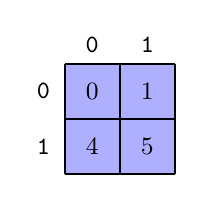
\begin{tikzpicture}[x={(0cm,-0.7cm)},y={(0.7cm,0cm)},every node/.style={minimum size=0.7cm, outer sep=0pt, font=\small}]
\node[fill={rgb,255:red,175;green,175;blue,255}] at (0,0) {0};
\node[fill={rgb,255:red,175;green,175;blue,255}] at (0,1) {1};
\node[fill={rgb,255:red,175;green,175;blue,255}] at (1,0) {4};
\node[fill={rgb,255:red,175;green,175;blue,255}] at (1,1) {5};
\draw[color=black,thick,step=0.7cm,shift={(-0.5,-0.5)}] (0,0) grid (2,2);
\node[anchor=east,minimum size=0pt] at (0,-0.6) {\texttt{0}};
\node[anchor=east,minimum size=0pt] at (1,-0.6) {\texttt{1}};
\node[minimum size=0pt] at (-0.85,0) {\texttt{0}};
\node[minimum size=0pt] at (-0.85,1) {\texttt{1}};
\end{tikzpicture}
\end{center}

and the two products are, with the element $(i,j)$ of $A$ as the row and the
copy $k$ as the column,
\begin{center}
\begin{minipage}[t]{0.48\linewidth}\centering
In CuTe: $A \otimes B$\\[4pt]
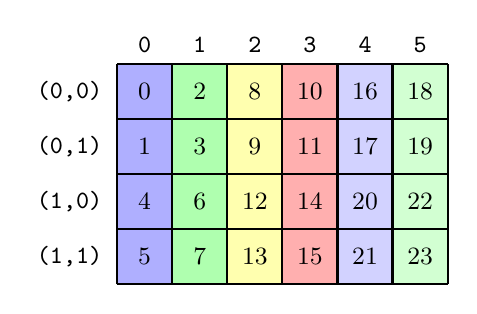
\begin{tikzpicture}[x={(0cm,-0.7cm)},y={(0.7cm,0cm)},every node/.style={minimum size=0.7cm, outer sep=0pt, font=\small}]
\node[fill={rgb,255:red,175;green,175;blue,255}] at (0,0) {0};
\node[fill={rgb,255:red,175;green,255;blue,175}] at (0,1) {2};
\node[fill={rgb,255:red,255;green,255;blue,175}] at (0,2) {8};
\node[fill={rgb,255:red,255;green,175;blue,175}] at (0,3) {10};
\node[fill={rgb,255:red,210;green,210;blue,255}] at (0,4) {16};
\node[fill={rgb,255:red,210;green,255;blue,210}] at (0,5) {18};
\node[fill={rgb,255:red,175;green,175;blue,255}] at (1,0) {1};
\node[fill={rgb,255:red,175;green,255;blue,175}] at (1,1) {3};
\node[fill={rgb,255:red,255;green,255;blue,175}] at (1,2) {9};
\node[fill={rgb,255:red,255;green,175;blue,175}] at (1,3) {11};
\node[fill={rgb,255:red,210;green,210;blue,255}] at (1,4) {17};
\node[fill={rgb,255:red,210;green,255;blue,210}] at (1,5) {19};
\node[fill={rgb,255:red,175;green,175;blue,255}] at (2,0) {4};
\node[fill={rgb,255:red,175;green,255;blue,175}] at (2,1) {6};
\node[fill={rgb,255:red,255;green,255;blue,175}] at (2,2) {12};
\node[fill={rgb,255:red,255;green,175;blue,175}] at (2,3) {14};
\node[fill={rgb,255:red,210;green,210;blue,255}] at (2,4) {20};
\node[fill={rgb,255:red,210;green,255;blue,210}] at (2,5) {22};
\node[fill={rgb,255:red,175;green,175;blue,255}] at (3,0) {5};
\node[fill={rgb,255:red,175;green,255;blue,175}] at (3,1) {7};
\node[fill={rgb,255:red,255;green,255;blue,175}] at (3,2) {13};
\node[fill={rgb,255:red,255;green,175;blue,175}] at (3,3) {15};
\node[fill={rgb,255:red,210;green,210;blue,255}] at (3,4) {21};
\node[fill={rgb,255:red,210;green,255;blue,210}] at (3,5) {23};
\draw[color=black,thick,step=0.7cm,shift={(-0.5,-0.5)}] (0,0) grid (4,6);
\node[anchor=east,minimum size=0pt] at (0,-0.6) {\texttt{(0,0)}};
\node[anchor=east,minimum size=0pt] at (1,-0.6) {\texttt{(0,1)}};
\node[anchor=east,minimum size=0pt] at (2,-0.6) {\texttt{(1,0)}};
\node[anchor=east,minimum size=0pt] at (3,-0.6) {\texttt{(1,1)}};
\node[minimum size=0pt] at (-0.85,0) {\texttt{0}};
\node[minimum size=0pt] at (-0.85,1) {\texttt{1}};
\node[minimum size=0pt] at (-0.85,2) {\texttt{2}};
\node[minimum size=0pt] at (-0.85,3) {\texttt{3}};
\node[minimum size=0pt] at (-0.85,4) {\texttt{4}};
\node[minimum size=0pt] at (-0.85,5) {\texttt{5}};
\end{tikzpicture}
\end{minipage}\hfill
\begin{minipage}[t]{0.48\linewidth}\centering
In our algebra: $\repeatop(A,B)$\\[4pt]
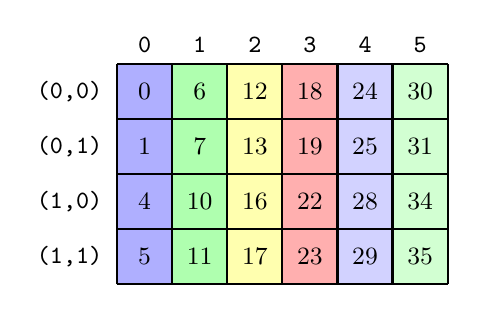
\begin{tikzpicture}[x={(0cm,-0.7cm)},y={(0.7cm,0cm)},every node/.style={minimum size=0.7cm, outer sep=0pt, font=\small}]
\node[fill={rgb,255:red,175;green,175;blue,255}] at (0,0) {0};
\node[fill={rgb,255:red,175;green,255;blue,175}] at (0,1) {6};
\node[fill={rgb,255:red,255;green,255;blue,175}] at (0,2) {12};
\node[fill={rgb,255:red,255;green,175;blue,175}] at (0,3) {18};
\node[fill={rgb,255:red,210;green,210;blue,255}] at (0,4) {24};
\node[fill={rgb,255:red,210;green,255;blue,210}] at (0,5) {30};
\node[fill={rgb,255:red,175;green,175;blue,255}] at (1,0) {1};
\node[fill={rgb,255:red,175;green,255;blue,175}] at (1,1) {7};
\node[fill={rgb,255:red,255;green,255;blue,175}] at (1,2) {13};
\node[fill={rgb,255:red,255;green,175;blue,175}] at (1,3) {19};
\node[fill={rgb,255:red,210;green,210;blue,255}] at (1,4) {25};
\node[fill={rgb,255:red,210;green,255;blue,210}] at (1,5) {31};
\node[fill={rgb,255:red,175;green,175;blue,255}] at (2,0) {4};
\node[fill={rgb,255:red,175;green,255;blue,175}] at (2,1) {10};
\node[fill={rgb,255:red,255;green,255;blue,175}] at (2,2) {16};
\node[fill={rgb,255:red,255;green,175;blue,175}] at (2,3) {22};
\node[fill={rgb,255:red,210;green,210;blue,255}] at (2,4) {28};
\node[fill={rgb,255:red,210;green,255;blue,210}] at (2,5) {34};
\node[fill={rgb,255:red,175;green,175;blue,255}] at (3,0) {5};
\node[fill={rgb,255:red,175;green,255;blue,175}] at (3,1) {11};
\node[fill={rgb,255:red,255;green,255;blue,175}] at (3,2) {17};
\node[fill={rgb,255:red,255;green,175;blue,175}] at (3,3) {23};
\node[fill={rgb,255:red,210;green,210;blue,255}] at (3,4) {29};
\node[fill={rgb,255:red,210;green,255;blue,210}] at (3,5) {35};
\draw[color=black,thick,step=0.7cm,shift={(-0.5,-0.5)}] (0,0) grid (4,6);
\node[anchor=east,minimum size=0pt] at (0,-0.6) {\texttt{(0,0)}};
\node[anchor=east,minimum size=0pt] at (1,-0.6) {\texttt{(0,1)}};
\node[anchor=east,minimum size=0pt] at (2,-0.6) {\texttt{(1,0)}};
\node[anchor=east,minimum size=0pt] at (3,-0.6) {\texttt{(1,1)}};
\node[minimum size=0pt] at (-0.85,0) {\texttt{0}};
\node[minimum size=0pt] at (-0.85,1) {\texttt{1}};
\node[minimum size=0pt] at (-0.85,2) {\texttt{2}};
\node[minimum size=0pt] at (-0.85,3) {\texttt{3}};
\node[minimum size=0pt] at (-0.85,4) {\texttt{4}};
\node[minimum size=0pt] at (-0.85,5) {\texttt{5}};
\end{tikzpicture}
\end{minipage}
\end{center}

In CuTe the copy offsets are $A^{*}_{24} = (2,3){:}(2,8)$, that is
$0, 2, 8, 10, 16, 18$, and
\[
A \otimes B = \big((2,2),(2,3)\big){:}\big((4,1),(2,8)\big)
\]
is a bijection onto $[0,24)$. In our algebra the copy offsets are the multiples of
$\cosize A = 6$, and $\repeatop(A,B) = (6,(2,2)){:}(6,(4,1))$ is injective and
not dense. CuTe's placement is available in our algebra:
$\divideop(\mathrm{canonical}(R), S)$ is the pair $(A, A^{*}_{M})$ of the
complement paragraph, and composing it on the right with
$\repeatop(B, \mathrm{canonical}(S_A))$, which sends $(a,b)$ to $(a, B(b))$,
gives $A \otimes B$ for every dense bijection $B$; for $B = k{:}1$ that
composition is the identity, and for this $A$
\[
A \otimes B = \divideop\big(\mathrm{canonical}((6,4)),\ (2,2)\big).
\]
All of this is checked. With the
operands exchanged and $B$ a dense bijection, $B \otimes A = (B,\
S_A{:}(\size B)\,D_A)$, which is $\interleave(A,B)$ up to the order of the
two coordinate groups. CuTe's \texttt{blocked\_product} and
\texttt{raked\_product} are both $A \otimes B$ with the two coordinate groups
zipped per mode, block index first or copy index first: the same map on
coordinates, regrouped. For $A = 4{:}1$ and $B = 2{:}1$, $A \otimes B =
\repeatop(A,B) = (2,4){:}(4,1)$, \texttt{raked\_product} is $(4,2){:}(1,4)$,
the same map with its two coordinates exchanged, and $B \otimes A =
\interleave(A,B) = (2,4){:}(1,2)$.

\paragraph{Conditions.} CuTe's six conditions exist because its composition
and complement must return a layout, so the operands are checked in advance
for the result to be expressible as one. In our algebra neither operation has
to: a composite is a map, and whether it is a layout is decided afterwards,
for code generation only; and a complement is never formed on its own, it is
the rest of a $\divideop$. So none of the six is checked. What is checked
instead is that the right operand of a composition is a dense bijection onto
the left operand's coordinates, by the stride criterion of
Lemma~\ref{lem:dense}; that a map into logical or thread-value space is a
dense bijection and a map into physical space is alias-free; and the
precondition of each operation, such as $k_i \mid n_i$ for $\divideop$.

\paragraph{Example.} Two hardware instructions and a kernel's use of them.
The thread-value maps are transcribed from the PTX ISA fragment
tables~\cite{ptx}. For
\texttt{mma.m16n8k16}, lane $4g + t_4$ holds four accumulator values
$(v_m, v_n)$, at row $g + 8v_m$ and column $2t_4 + v_n$ of the $16 \times 8$
tile; with the tile row-major,
\[
F_C = \big((8,4),(2,2)\big){:}\big((8,2),(64,1)\big) : \tv \to \logical .
\]
For \texttt{ldmatrix}, lane $4g + q$ holds elements $(g, 2q)$ and $(g, 2q+1)$
of an $8 \times 8$ matrix,
\[
F_{\mathrm{ld}} = \big((8,4),2\big){:}\big((8,2),1\big) : \tv \to \logical .
\]
Printed as CuTe prints thread-value layouts, one cell per element of the tile,
labelled with the lane and value that hold it and coloured by lane:
\begin{center}
\begin{minipage}[t]{0.42\linewidth}\centering
$F_C$: the $16 \times 8$ accumulator\\[4pt]
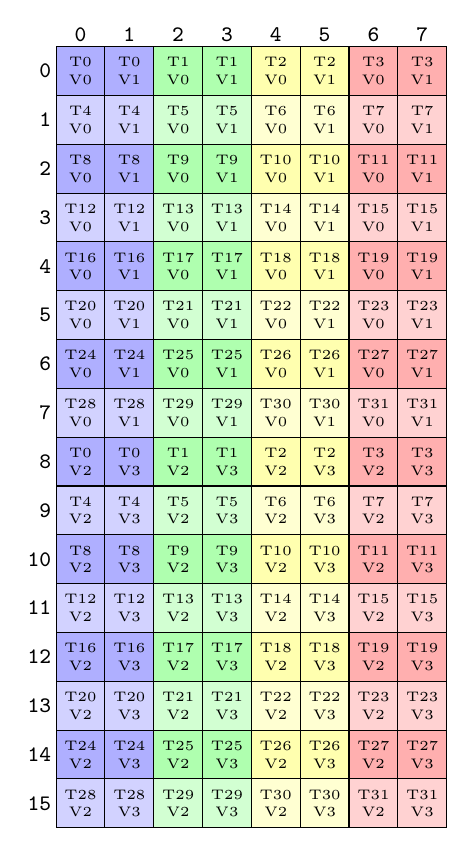
\begin{tikzpicture}[x={(0cm,-0.62cm)},y={(0.62cm,0cm)},every node/.style={minimum size=0.62cm, outer sep=0pt, inner sep=0pt, font=\tiny}]
\node[fill={rgb,255:red,175;green,175;blue,255}] at (0,0) {\shortstack{T0\\V0}};
\node[fill={rgb,255:red,175;green,175;blue,255}] at (0,1) {\shortstack{T0\\V1}};
\node[fill={rgb,255:red,175;green,255;blue,175}] at (0,2) {\shortstack{T1\\V0}};
\node[fill={rgb,255:red,175;green,255;blue,175}] at (0,3) {\shortstack{T1\\V1}};
\node[fill={rgb,255:red,255;green,255;blue,175}] at (0,4) {\shortstack{T2\\V0}};
\node[fill={rgb,255:red,255;green,255;blue,175}] at (0,5) {\shortstack{T2\\V1}};
\node[fill={rgb,255:red,255;green,175;blue,175}] at (0,6) {\shortstack{T3\\V0}};
\node[fill={rgb,255:red,255;green,175;blue,175}] at (0,7) {\shortstack{T3\\V1}};
\node[fill={rgb,255:red,210;green,210;blue,255}] at (1,0) {\shortstack{T4\\V0}};
\node[fill={rgb,255:red,210;green,210;blue,255}] at (1,1) {\shortstack{T4\\V1}};
\node[fill={rgb,255:red,210;green,255;blue,210}] at (1,2) {\shortstack{T5\\V0}};
\node[fill={rgb,255:red,210;green,255;blue,210}] at (1,3) {\shortstack{T5\\V1}};
\node[fill={rgb,255:red,255;green,255;blue,210}] at (1,4) {\shortstack{T6\\V0}};
\node[fill={rgb,255:red,255;green,255;blue,210}] at (1,5) {\shortstack{T6\\V1}};
\node[fill={rgb,255:red,255;green,210;blue,210}] at (1,6) {\shortstack{T7\\V0}};
\node[fill={rgb,255:red,255;green,210;blue,210}] at (1,7) {\shortstack{T7\\V1}};
\node[fill={rgb,255:red,175;green,175;blue,255}] at (2,0) {\shortstack{T8\\V0}};
\node[fill={rgb,255:red,175;green,175;blue,255}] at (2,1) {\shortstack{T8\\V1}};
\node[fill={rgb,255:red,175;green,255;blue,175}] at (2,2) {\shortstack{T9\\V0}};
\node[fill={rgb,255:red,175;green,255;blue,175}] at (2,3) {\shortstack{T9\\V1}};
\node[fill={rgb,255:red,255;green,255;blue,175}] at (2,4) {\shortstack{T10\\V0}};
\node[fill={rgb,255:red,255;green,255;blue,175}] at (2,5) {\shortstack{T10\\V1}};
\node[fill={rgb,255:red,255;green,175;blue,175}] at (2,6) {\shortstack{T11\\V0}};
\node[fill={rgb,255:red,255;green,175;blue,175}] at (2,7) {\shortstack{T11\\V1}};
\node[fill={rgb,255:red,210;green,210;blue,255}] at (3,0) {\shortstack{T12\\V0}};
\node[fill={rgb,255:red,210;green,210;blue,255}] at (3,1) {\shortstack{T12\\V1}};
\node[fill={rgb,255:red,210;green,255;blue,210}] at (3,2) {\shortstack{T13\\V0}};
\node[fill={rgb,255:red,210;green,255;blue,210}] at (3,3) {\shortstack{T13\\V1}};
\node[fill={rgb,255:red,255;green,255;blue,210}] at (3,4) {\shortstack{T14\\V0}};
\node[fill={rgb,255:red,255;green,255;blue,210}] at (3,5) {\shortstack{T14\\V1}};
\node[fill={rgb,255:red,255;green,210;blue,210}] at (3,6) {\shortstack{T15\\V0}};
\node[fill={rgb,255:red,255;green,210;blue,210}] at (3,7) {\shortstack{T15\\V1}};
\node[fill={rgb,255:red,175;green,175;blue,255}] at (4,0) {\shortstack{T16\\V0}};
\node[fill={rgb,255:red,175;green,175;blue,255}] at (4,1) {\shortstack{T16\\V1}};
\node[fill={rgb,255:red,175;green,255;blue,175}] at (4,2) {\shortstack{T17\\V0}};
\node[fill={rgb,255:red,175;green,255;blue,175}] at (4,3) {\shortstack{T17\\V1}};
\node[fill={rgb,255:red,255;green,255;blue,175}] at (4,4) {\shortstack{T18\\V0}};
\node[fill={rgb,255:red,255;green,255;blue,175}] at (4,5) {\shortstack{T18\\V1}};
\node[fill={rgb,255:red,255;green,175;blue,175}] at (4,6) {\shortstack{T19\\V0}};
\node[fill={rgb,255:red,255;green,175;blue,175}] at (4,7) {\shortstack{T19\\V1}};
\node[fill={rgb,255:red,210;green,210;blue,255}] at (5,0) {\shortstack{T20\\V0}};
\node[fill={rgb,255:red,210;green,210;blue,255}] at (5,1) {\shortstack{T20\\V1}};
\node[fill={rgb,255:red,210;green,255;blue,210}] at (5,2) {\shortstack{T21\\V0}};
\node[fill={rgb,255:red,210;green,255;blue,210}] at (5,3) {\shortstack{T21\\V1}};
\node[fill={rgb,255:red,255;green,255;blue,210}] at (5,4) {\shortstack{T22\\V0}};
\node[fill={rgb,255:red,255;green,255;blue,210}] at (5,5) {\shortstack{T22\\V1}};
\node[fill={rgb,255:red,255;green,210;blue,210}] at (5,6) {\shortstack{T23\\V0}};
\node[fill={rgb,255:red,255;green,210;blue,210}] at (5,7) {\shortstack{T23\\V1}};
\node[fill={rgb,255:red,175;green,175;blue,255}] at (6,0) {\shortstack{T24\\V0}};
\node[fill={rgb,255:red,175;green,175;blue,255}] at (6,1) {\shortstack{T24\\V1}};
\node[fill={rgb,255:red,175;green,255;blue,175}] at (6,2) {\shortstack{T25\\V0}};
\node[fill={rgb,255:red,175;green,255;blue,175}] at (6,3) {\shortstack{T25\\V1}};
\node[fill={rgb,255:red,255;green,255;blue,175}] at (6,4) {\shortstack{T26\\V0}};
\node[fill={rgb,255:red,255;green,255;blue,175}] at (6,5) {\shortstack{T26\\V1}};
\node[fill={rgb,255:red,255;green,175;blue,175}] at (6,6) {\shortstack{T27\\V0}};
\node[fill={rgb,255:red,255;green,175;blue,175}] at (6,7) {\shortstack{T27\\V1}};
\node[fill={rgb,255:red,210;green,210;blue,255}] at (7,0) {\shortstack{T28\\V0}};
\node[fill={rgb,255:red,210;green,210;blue,255}] at (7,1) {\shortstack{T28\\V1}};
\node[fill={rgb,255:red,210;green,255;blue,210}] at (7,2) {\shortstack{T29\\V0}};
\node[fill={rgb,255:red,210;green,255;blue,210}] at (7,3) {\shortstack{T29\\V1}};
\node[fill={rgb,255:red,255;green,255;blue,210}] at (7,4) {\shortstack{T30\\V0}};
\node[fill={rgb,255:red,255;green,255;blue,210}] at (7,5) {\shortstack{T30\\V1}};
\node[fill={rgb,255:red,255;green,210;blue,210}] at (7,6) {\shortstack{T31\\V0}};
\node[fill={rgb,255:red,255;green,210;blue,210}] at (7,7) {\shortstack{T31\\V1}};
\node[fill={rgb,255:red,175;green,175;blue,255}] at (8,0) {\shortstack{T0\\V2}};
\node[fill={rgb,255:red,175;green,175;blue,255}] at (8,1) {\shortstack{T0\\V3}};
\node[fill={rgb,255:red,175;green,255;blue,175}] at (8,2) {\shortstack{T1\\V2}};
\node[fill={rgb,255:red,175;green,255;blue,175}] at (8,3) {\shortstack{T1\\V3}};
\node[fill={rgb,255:red,255;green,255;blue,175}] at (8,4) {\shortstack{T2\\V2}};
\node[fill={rgb,255:red,255;green,255;blue,175}] at (8,5) {\shortstack{T2\\V3}};
\node[fill={rgb,255:red,255;green,175;blue,175}] at (8,6) {\shortstack{T3\\V2}};
\node[fill={rgb,255:red,255;green,175;blue,175}] at (8,7) {\shortstack{T3\\V3}};
\node[fill={rgb,255:red,210;green,210;blue,255}] at (9,0) {\shortstack{T4\\V2}};
\node[fill={rgb,255:red,210;green,210;blue,255}] at (9,1) {\shortstack{T4\\V3}};
\node[fill={rgb,255:red,210;green,255;blue,210}] at (9,2) {\shortstack{T5\\V2}};
\node[fill={rgb,255:red,210;green,255;blue,210}] at (9,3) {\shortstack{T5\\V3}};
\node[fill={rgb,255:red,255;green,255;blue,210}] at (9,4) {\shortstack{T6\\V2}};
\node[fill={rgb,255:red,255;green,255;blue,210}] at (9,5) {\shortstack{T6\\V3}};
\node[fill={rgb,255:red,255;green,210;blue,210}] at (9,6) {\shortstack{T7\\V2}};
\node[fill={rgb,255:red,255;green,210;blue,210}] at (9,7) {\shortstack{T7\\V3}};
\node[fill={rgb,255:red,175;green,175;blue,255}] at (10,0) {\shortstack{T8\\V2}};
\node[fill={rgb,255:red,175;green,175;blue,255}] at (10,1) {\shortstack{T8\\V3}};
\node[fill={rgb,255:red,175;green,255;blue,175}] at (10,2) {\shortstack{T9\\V2}};
\node[fill={rgb,255:red,175;green,255;blue,175}] at (10,3) {\shortstack{T9\\V3}};
\node[fill={rgb,255:red,255;green,255;blue,175}] at (10,4) {\shortstack{T10\\V2}};
\node[fill={rgb,255:red,255;green,255;blue,175}] at (10,5) {\shortstack{T10\\V3}};
\node[fill={rgb,255:red,255;green,175;blue,175}] at (10,6) {\shortstack{T11\\V2}};
\node[fill={rgb,255:red,255;green,175;blue,175}] at (10,7) {\shortstack{T11\\V3}};
\node[fill={rgb,255:red,210;green,210;blue,255}] at (11,0) {\shortstack{T12\\V2}};
\node[fill={rgb,255:red,210;green,210;blue,255}] at (11,1) {\shortstack{T12\\V3}};
\node[fill={rgb,255:red,210;green,255;blue,210}] at (11,2) {\shortstack{T13\\V2}};
\node[fill={rgb,255:red,210;green,255;blue,210}] at (11,3) {\shortstack{T13\\V3}};
\node[fill={rgb,255:red,255;green,255;blue,210}] at (11,4) {\shortstack{T14\\V2}};
\node[fill={rgb,255:red,255;green,255;blue,210}] at (11,5) {\shortstack{T14\\V3}};
\node[fill={rgb,255:red,255;green,210;blue,210}] at (11,6) {\shortstack{T15\\V2}};
\node[fill={rgb,255:red,255;green,210;blue,210}] at (11,7) {\shortstack{T15\\V3}};
\node[fill={rgb,255:red,175;green,175;blue,255}] at (12,0) {\shortstack{T16\\V2}};
\node[fill={rgb,255:red,175;green,175;blue,255}] at (12,1) {\shortstack{T16\\V3}};
\node[fill={rgb,255:red,175;green,255;blue,175}] at (12,2) {\shortstack{T17\\V2}};
\node[fill={rgb,255:red,175;green,255;blue,175}] at (12,3) {\shortstack{T17\\V3}};
\node[fill={rgb,255:red,255;green,255;blue,175}] at (12,4) {\shortstack{T18\\V2}};
\node[fill={rgb,255:red,255;green,255;blue,175}] at (12,5) {\shortstack{T18\\V3}};
\node[fill={rgb,255:red,255;green,175;blue,175}] at (12,6) {\shortstack{T19\\V2}};
\node[fill={rgb,255:red,255;green,175;blue,175}] at (12,7) {\shortstack{T19\\V3}};
\node[fill={rgb,255:red,210;green,210;blue,255}] at (13,0) {\shortstack{T20\\V2}};
\node[fill={rgb,255:red,210;green,210;blue,255}] at (13,1) {\shortstack{T20\\V3}};
\node[fill={rgb,255:red,210;green,255;blue,210}] at (13,2) {\shortstack{T21\\V2}};
\node[fill={rgb,255:red,210;green,255;blue,210}] at (13,3) {\shortstack{T21\\V3}};
\node[fill={rgb,255:red,255;green,255;blue,210}] at (13,4) {\shortstack{T22\\V2}};
\node[fill={rgb,255:red,255;green,255;blue,210}] at (13,5) {\shortstack{T22\\V3}};
\node[fill={rgb,255:red,255;green,210;blue,210}] at (13,6) {\shortstack{T23\\V2}};
\node[fill={rgb,255:red,255;green,210;blue,210}] at (13,7) {\shortstack{T23\\V3}};
\node[fill={rgb,255:red,175;green,175;blue,255}] at (14,0) {\shortstack{T24\\V2}};
\node[fill={rgb,255:red,175;green,175;blue,255}] at (14,1) {\shortstack{T24\\V3}};
\node[fill={rgb,255:red,175;green,255;blue,175}] at (14,2) {\shortstack{T25\\V2}};
\node[fill={rgb,255:red,175;green,255;blue,175}] at (14,3) {\shortstack{T25\\V3}};
\node[fill={rgb,255:red,255;green,255;blue,175}] at (14,4) {\shortstack{T26\\V2}};
\node[fill={rgb,255:red,255;green,255;blue,175}] at (14,5) {\shortstack{T26\\V3}};
\node[fill={rgb,255:red,255;green,175;blue,175}] at (14,6) {\shortstack{T27\\V2}};
\node[fill={rgb,255:red,255;green,175;blue,175}] at (14,7) {\shortstack{T27\\V3}};
\node[fill={rgb,255:red,210;green,210;blue,255}] at (15,0) {\shortstack{T28\\V2}};
\node[fill={rgb,255:red,210;green,210;blue,255}] at (15,1) {\shortstack{T28\\V3}};
\node[fill={rgb,255:red,210;green,255;blue,210}] at (15,2) {\shortstack{T29\\V2}};
\node[fill={rgb,255:red,210;green,255;blue,210}] at (15,3) {\shortstack{T29\\V3}};
\node[fill={rgb,255:red,255;green,255;blue,210}] at (15,4) {\shortstack{T30\\V2}};
\node[fill={rgb,255:red,255;green,255;blue,210}] at (15,5) {\shortstack{T30\\V3}};
\node[fill={rgb,255:red,255;green,210;blue,210}] at (15,6) {\shortstack{T31\\V2}};
\node[fill={rgb,255:red,255;green,210;blue,210}] at (15,7) {\shortstack{T31\\V3}};
\draw[color=black,thin,step=0.62cm,shift={(-0.5,-0.5)}] (0,0) grid (16,8);
\node[anchor=east,minimum size=0pt,font=\footnotesize] at (0,-0.6) {\texttt{0}};
\node[anchor=east,minimum size=0pt,font=\footnotesize] at (1,-0.6) {\texttt{1}};
\node[anchor=east,minimum size=0pt,font=\footnotesize] at (2,-0.6) {\texttt{2}};
\node[anchor=east,minimum size=0pt,font=\footnotesize] at (3,-0.6) {\texttt{3}};
\node[anchor=east,minimum size=0pt,font=\footnotesize] at (4,-0.6) {\texttt{4}};
\node[anchor=east,minimum size=0pt,font=\footnotesize] at (5,-0.6) {\texttt{5}};
\node[anchor=east,minimum size=0pt,font=\footnotesize] at (6,-0.6) {\texttt{6}};
\node[anchor=east,minimum size=0pt,font=\footnotesize] at (7,-0.6) {\texttt{7}};
\node[anchor=east,minimum size=0pt,font=\footnotesize] at (8,-0.6) {\texttt{8}};
\node[anchor=east,minimum size=0pt,font=\footnotesize] at (9,-0.6) {\texttt{9}};
\node[anchor=east,minimum size=0pt,font=\footnotesize] at (10,-0.6) {\texttt{10}};
\node[anchor=east,minimum size=0pt,font=\footnotesize] at (11,-0.6) {\texttt{11}};
\node[anchor=east,minimum size=0pt,font=\footnotesize] at (12,-0.6) {\texttt{12}};
\node[anchor=east,minimum size=0pt,font=\footnotesize] at (13,-0.6) {\texttt{13}};
\node[anchor=east,minimum size=0pt,font=\footnotesize] at (14,-0.6) {\texttt{14}};
\node[anchor=east,minimum size=0pt,font=\footnotesize] at (15,-0.6) {\texttt{15}};
\node[minimum size=0pt,font=\footnotesize] at (-0.75,0) {\texttt{0}};
\node[minimum size=0pt,font=\footnotesize] at (-0.75,1) {\texttt{1}};
\node[minimum size=0pt,font=\footnotesize] at (-0.75,2) {\texttt{2}};
\node[minimum size=0pt,font=\footnotesize] at (-0.75,3) {\texttt{3}};
\node[minimum size=0pt,font=\footnotesize] at (-0.75,4) {\texttt{4}};
\node[minimum size=0pt,font=\footnotesize] at (-0.75,5) {\texttt{5}};
\node[minimum size=0pt,font=\footnotesize] at (-0.75,6) {\texttt{6}};
\node[minimum size=0pt,font=\footnotesize] at (-0.75,7) {\texttt{7}};
\end{tikzpicture}
\end{minipage}\hfill
\begin{minipage}[t]{0.42\linewidth}\centering
$F_{\mathrm{ld}}$: one $8 \times 8$ matrix\\[4pt]
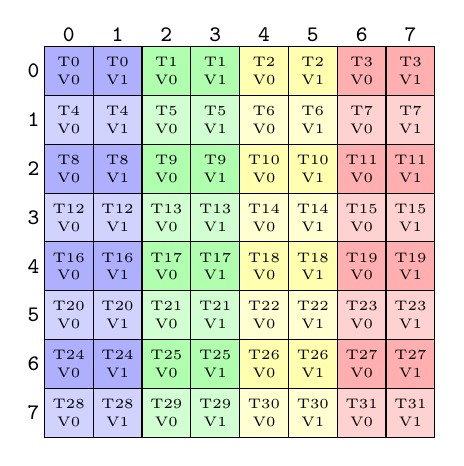
\begin{tikzpicture}[x={(0cm,-0.62cm)},y={(0.62cm,0cm)},every node/.style={minimum size=0.62cm, outer sep=0pt, inner sep=0pt, font=\tiny}]
\node[fill={rgb,255:red,175;green,175;blue,255}] at (0,0) {\shortstack{T0\\V0}};
\node[fill={rgb,255:red,175;green,175;blue,255}] at (0,1) {\shortstack{T0\\V1}};
\node[fill={rgb,255:red,175;green,255;blue,175}] at (0,2) {\shortstack{T1\\V0}};
\node[fill={rgb,255:red,175;green,255;blue,175}] at (0,3) {\shortstack{T1\\V1}};
\node[fill={rgb,255:red,255;green,255;blue,175}] at (0,4) {\shortstack{T2\\V0}};
\node[fill={rgb,255:red,255;green,255;blue,175}] at (0,5) {\shortstack{T2\\V1}};
\node[fill={rgb,255:red,255;green,175;blue,175}] at (0,6) {\shortstack{T3\\V0}};
\node[fill={rgb,255:red,255;green,175;blue,175}] at (0,7) {\shortstack{T3\\V1}};
\node[fill={rgb,255:red,210;green,210;blue,255}] at (1,0) {\shortstack{T4\\V0}};
\node[fill={rgb,255:red,210;green,210;blue,255}] at (1,1) {\shortstack{T4\\V1}};
\node[fill={rgb,255:red,210;green,255;blue,210}] at (1,2) {\shortstack{T5\\V0}};
\node[fill={rgb,255:red,210;green,255;blue,210}] at (1,3) {\shortstack{T5\\V1}};
\node[fill={rgb,255:red,255;green,255;blue,210}] at (1,4) {\shortstack{T6\\V0}};
\node[fill={rgb,255:red,255;green,255;blue,210}] at (1,5) {\shortstack{T6\\V1}};
\node[fill={rgb,255:red,255;green,210;blue,210}] at (1,6) {\shortstack{T7\\V0}};
\node[fill={rgb,255:red,255;green,210;blue,210}] at (1,7) {\shortstack{T7\\V1}};
\node[fill={rgb,255:red,175;green,175;blue,255}] at (2,0) {\shortstack{T8\\V0}};
\node[fill={rgb,255:red,175;green,175;blue,255}] at (2,1) {\shortstack{T8\\V1}};
\node[fill={rgb,255:red,175;green,255;blue,175}] at (2,2) {\shortstack{T9\\V0}};
\node[fill={rgb,255:red,175;green,255;blue,175}] at (2,3) {\shortstack{T9\\V1}};
\node[fill={rgb,255:red,255;green,255;blue,175}] at (2,4) {\shortstack{T10\\V0}};
\node[fill={rgb,255:red,255;green,255;blue,175}] at (2,5) {\shortstack{T10\\V1}};
\node[fill={rgb,255:red,255;green,175;blue,175}] at (2,6) {\shortstack{T11\\V0}};
\node[fill={rgb,255:red,255;green,175;blue,175}] at (2,7) {\shortstack{T11\\V1}};
\node[fill={rgb,255:red,210;green,210;blue,255}] at (3,0) {\shortstack{T12\\V0}};
\node[fill={rgb,255:red,210;green,210;blue,255}] at (3,1) {\shortstack{T12\\V1}};
\node[fill={rgb,255:red,210;green,255;blue,210}] at (3,2) {\shortstack{T13\\V0}};
\node[fill={rgb,255:red,210;green,255;blue,210}] at (3,3) {\shortstack{T13\\V1}};
\node[fill={rgb,255:red,255;green,255;blue,210}] at (3,4) {\shortstack{T14\\V0}};
\node[fill={rgb,255:red,255;green,255;blue,210}] at (3,5) {\shortstack{T14\\V1}};
\node[fill={rgb,255:red,255;green,210;blue,210}] at (3,6) {\shortstack{T15\\V0}};
\node[fill={rgb,255:red,255;green,210;blue,210}] at (3,7) {\shortstack{T15\\V1}};
\node[fill={rgb,255:red,175;green,175;blue,255}] at (4,0) {\shortstack{T16\\V0}};
\node[fill={rgb,255:red,175;green,175;blue,255}] at (4,1) {\shortstack{T16\\V1}};
\node[fill={rgb,255:red,175;green,255;blue,175}] at (4,2) {\shortstack{T17\\V0}};
\node[fill={rgb,255:red,175;green,255;blue,175}] at (4,3) {\shortstack{T17\\V1}};
\node[fill={rgb,255:red,255;green,255;blue,175}] at (4,4) {\shortstack{T18\\V0}};
\node[fill={rgb,255:red,255;green,255;blue,175}] at (4,5) {\shortstack{T18\\V1}};
\node[fill={rgb,255:red,255;green,175;blue,175}] at (4,6) {\shortstack{T19\\V0}};
\node[fill={rgb,255:red,255;green,175;blue,175}] at (4,7) {\shortstack{T19\\V1}};
\node[fill={rgb,255:red,210;green,210;blue,255}] at (5,0) {\shortstack{T20\\V0}};
\node[fill={rgb,255:red,210;green,210;blue,255}] at (5,1) {\shortstack{T20\\V1}};
\node[fill={rgb,255:red,210;green,255;blue,210}] at (5,2) {\shortstack{T21\\V0}};
\node[fill={rgb,255:red,210;green,255;blue,210}] at (5,3) {\shortstack{T21\\V1}};
\node[fill={rgb,255:red,255;green,255;blue,210}] at (5,4) {\shortstack{T22\\V0}};
\node[fill={rgb,255:red,255;green,255;blue,210}] at (5,5) {\shortstack{T22\\V1}};
\node[fill={rgb,255:red,255;green,210;blue,210}] at (5,6) {\shortstack{T23\\V0}};
\node[fill={rgb,255:red,255;green,210;blue,210}] at (5,7) {\shortstack{T23\\V1}};
\node[fill={rgb,255:red,175;green,175;blue,255}] at (6,0) {\shortstack{T24\\V0}};
\node[fill={rgb,255:red,175;green,175;blue,255}] at (6,1) {\shortstack{T24\\V1}};
\node[fill={rgb,255:red,175;green,255;blue,175}] at (6,2) {\shortstack{T25\\V0}};
\node[fill={rgb,255:red,175;green,255;blue,175}] at (6,3) {\shortstack{T25\\V1}};
\node[fill={rgb,255:red,255;green,255;blue,175}] at (6,4) {\shortstack{T26\\V0}};
\node[fill={rgb,255:red,255;green,255;blue,175}] at (6,5) {\shortstack{T26\\V1}};
\node[fill={rgb,255:red,255;green,175;blue,175}] at (6,6) {\shortstack{T27\\V0}};
\node[fill={rgb,255:red,255;green,175;blue,175}] at (6,7) {\shortstack{T27\\V1}};
\node[fill={rgb,255:red,210;green,210;blue,255}] at (7,0) {\shortstack{T28\\V0}};
\node[fill={rgb,255:red,210;green,210;blue,255}] at (7,1) {\shortstack{T28\\V1}};
\node[fill={rgb,255:red,210;green,255;blue,210}] at (7,2) {\shortstack{T29\\V0}};
\node[fill={rgb,255:red,210;green,255;blue,210}] at (7,3) {\shortstack{T29\\V1}};
\node[fill={rgb,255:red,255;green,255;blue,210}] at (7,4) {\shortstack{T30\\V0}};
\node[fill={rgb,255:red,255;green,255;blue,210}] at (7,5) {\shortstack{T30\\V1}};
\node[fill={rgb,255:red,255;green,210;blue,210}] at (7,6) {\shortstack{T31\\V0}};
\node[fill={rgb,255:red,255;green,210;blue,210}] at (7,7) {\shortstack{T31\\V1}};
\draw[color=black,thin,step=0.62cm,shift={(-0.5,-0.5)}] (0,0) grid (8,8);
\node[anchor=east,minimum size=0pt,font=\footnotesize] at (0,-0.6) {\texttt{0}};
\node[anchor=east,minimum size=0pt,font=\footnotesize] at (1,-0.6) {\texttt{1}};
\node[anchor=east,minimum size=0pt,font=\footnotesize] at (2,-0.6) {\texttt{2}};
\node[anchor=east,minimum size=0pt,font=\footnotesize] at (3,-0.6) {\texttt{3}};
\node[anchor=east,minimum size=0pt,font=\footnotesize] at (4,-0.6) {\texttt{4}};
\node[anchor=east,minimum size=0pt,font=\footnotesize] at (5,-0.6) {\texttt{5}};
\node[anchor=east,minimum size=0pt,font=\footnotesize] at (6,-0.6) {\texttt{6}};
\node[anchor=east,minimum size=0pt,font=\footnotesize] at (7,-0.6) {\texttt{7}};
\node[minimum size=0pt,font=\footnotesize] at (-0.75,0) {\texttt{0}};
\node[minimum size=0pt,font=\footnotesize] at (-0.75,1) {\texttt{1}};
\node[minimum size=0pt,font=\footnotesize] at (-0.75,2) {\texttt{2}};
\node[minimum size=0pt,font=\footnotesize] at (-0.75,3) {\texttt{3}};
\node[minimum size=0pt,font=\footnotesize] at (-0.75,4) {\texttt{4}};
\node[minimum size=0pt,font=\footnotesize] at (-0.75,5) {\texttt{5}};
\node[minimum size=0pt,font=\footnotesize] at (-0.75,6) {\texttt{6}};
\node[minimum size=0pt,font=\footnotesize] at (-0.75,7) {\texttt{7}};
\end{tikzpicture}
\end{minipage}
\end{center}

A kernel uses them through the operations. Two warps, $W = 2{:}1$, computing
a $16 \times 16$ tile side by side have the thread-value map
\[
\divideop\big(\mathrm{canonical}((16,16)),\ (16,8)\big) \circ \interleave(F_C, W),
\]
with domain $(\text{warp}, (\text{lane}, \text{value}))$, and one warp loading
the four $8 \times 8$ matrices of an $8 \times 32$ tile with
\texttt{ldmatrix.x4} has
\[
\divideop\big(\mathrm{canonical}((8,32)),\ (8,8)\big) \circ \interleave(F_{\mathrm{ld}}, 4{:}1),
\]
with domain $(\text{matrix}, (\text{lane}, \text{value}))$. Coloured by warp
and by matrix respectively; in the first, cells are labelled by the thread
$32w + \text{lane}$:
\begin{center}
two warps on $16 \times 16$\\[4pt]
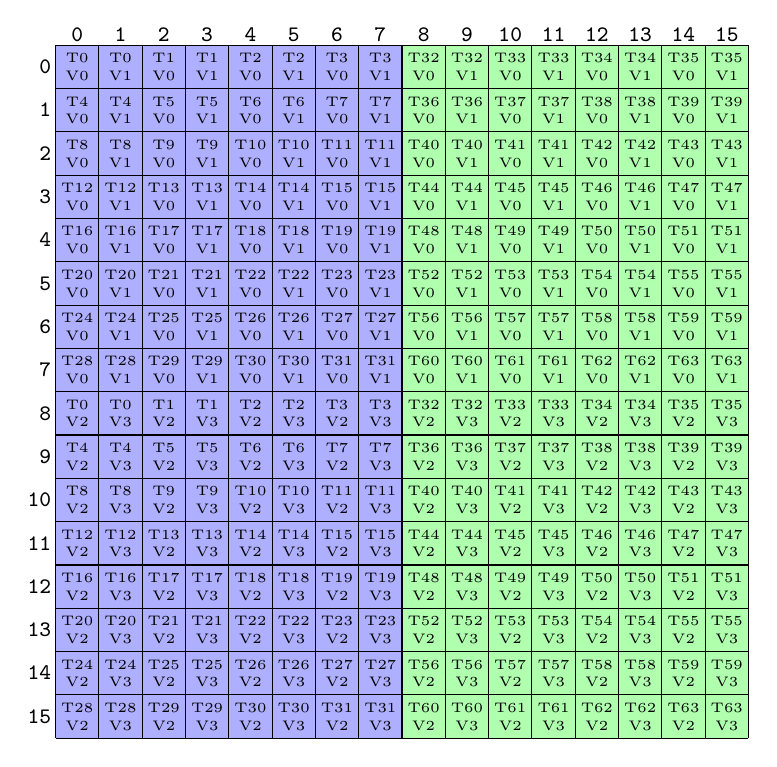
\begin{tikzpicture}[x={(0cm,-0.55cm)},y={(0.55cm,0cm)},every node/.style={minimum size=0.55cm, outer sep=0pt, inner sep=0pt, font=\tiny}]
\node[fill={rgb,255:red,175;green,175;blue,255}] at (0,0) {\shortstack{T0\\V0}};
\node[fill={rgb,255:red,175;green,175;blue,255}] at (0,1) {\shortstack{T0\\V1}};
\node[fill={rgb,255:red,175;green,175;blue,255}] at (0,2) {\shortstack{T1\\V0}};
\node[fill={rgb,255:red,175;green,175;blue,255}] at (0,3) {\shortstack{T1\\V1}};
\node[fill={rgb,255:red,175;green,175;blue,255}] at (0,4) {\shortstack{T2\\V0}};
\node[fill={rgb,255:red,175;green,175;blue,255}] at (0,5) {\shortstack{T2\\V1}};
\node[fill={rgb,255:red,175;green,175;blue,255}] at (0,6) {\shortstack{T3\\V0}};
\node[fill={rgb,255:red,175;green,175;blue,255}] at (0,7) {\shortstack{T3\\V1}};
\node[fill={rgb,255:red,175;green,255;blue,175}] at (0,8) {\shortstack{T32\\V0}};
\node[fill={rgb,255:red,175;green,255;blue,175}] at (0,9) {\shortstack{T32\\V1}};
\node[fill={rgb,255:red,175;green,255;blue,175}] at (0,10) {\shortstack{T33\\V0}};
\node[fill={rgb,255:red,175;green,255;blue,175}] at (0,11) {\shortstack{T33\\V1}};
\node[fill={rgb,255:red,175;green,255;blue,175}] at (0,12) {\shortstack{T34\\V0}};
\node[fill={rgb,255:red,175;green,255;blue,175}] at (0,13) {\shortstack{T34\\V1}};
\node[fill={rgb,255:red,175;green,255;blue,175}] at (0,14) {\shortstack{T35\\V0}};
\node[fill={rgb,255:red,175;green,255;blue,175}] at (0,15) {\shortstack{T35\\V1}};
\node[fill={rgb,255:red,175;green,175;blue,255}] at (1,0) {\shortstack{T4\\V0}};
\node[fill={rgb,255:red,175;green,175;blue,255}] at (1,1) {\shortstack{T4\\V1}};
\node[fill={rgb,255:red,175;green,175;blue,255}] at (1,2) {\shortstack{T5\\V0}};
\node[fill={rgb,255:red,175;green,175;blue,255}] at (1,3) {\shortstack{T5\\V1}};
\node[fill={rgb,255:red,175;green,175;blue,255}] at (1,4) {\shortstack{T6\\V0}};
\node[fill={rgb,255:red,175;green,175;blue,255}] at (1,5) {\shortstack{T6\\V1}};
\node[fill={rgb,255:red,175;green,175;blue,255}] at (1,6) {\shortstack{T7\\V0}};
\node[fill={rgb,255:red,175;green,175;blue,255}] at (1,7) {\shortstack{T7\\V1}};
\node[fill={rgb,255:red,175;green,255;blue,175}] at (1,8) {\shortstack{T36\\V0}};
\node[fill={rgb,255:red,175;green,255;blue,175}] at (1,9) {\shortstack{T36\\V1}};
\node[fill={rgb,255:red,175;green,255;blue,175}] at (1,10) {\shortstack{T37\\V0}};
\node[fill={rgb,255:red,175;green,255;blue,175}] at (1,11) {\shortstack{T37\\V1}};
\node[fill={rgb,255:red,175;green,255;blue,175}] at (1,12) {\shortstack{T38\\V0}};
\node[fill={rgb,255:red,175;green,255;blue,175}] at (1,13) {\shortstack{T38\\V1}};
\node[fill={rgb,255:red,175;green,255;blue,175}] at (1,14) {\shortstack{T39\\V0}};
\node[fill={rgb,255:red,175;green,255;blue,175}] at (1,15) {\shortstack{T39\\V1}};
\node[fill={rgb,255:red,175;green,175;blue,255}] at (2,0) {\shortstack{T8\\V0}};
\node[fill={rgb,255:red,175;green,175;blue,255}] at (2,1) {\shortstack{T8\\V1}};
\node[fill={rgb,255:red,175;green,175;blue,255}] at (2,2) {\shortstack{T9\\V0}};
\node[fill={rgb,255:red,175;green,175;blue,255}] at (2,3) {\shortstack{T9\\V1}};
\node[fill={rgb,255:red,175;green,175;blue,255}] at (2,4) {\shortstack{T10\\V0}};
\node[fill={rgb,255:red,175;green,175;blue,255}] at (2,5) {\shortstack{T10\\V1}};
\node[fill={rgb,255:red,175;green,175;blue,255}] at (2,6) {\shortstack{T11\\V0}};
\node[fill={rgb,255:red,175;green,175;blue,255}] at (2,7) {\shortstack{T11\\V1}};
\node[fill={rgb,255:red,175;green,255;blue,175}] at (2,8) {\shortstack{T40\\V0}};
\node[fill={rgb,255:red,175;green,255;blue,175}] at (2,9) {\shortstack{T40\\V1}};
\node[fill={rgb,255:red,175;green,255;blue,175}] at (2,10) {\shortstack{T41\\V0}};
\node[fill={rgb,255:red,175;green,255;blue,175}] at (2,11) {\shortstack{T41\\V1}};
\node[fill={rgb,255:red,175;green,255;blue,175}] at (2,12) {\shortstack{T42\\V0}};
\node[fill={rgb,255:red,175;green,255;blue,175}] at (2,13) {\shortstack{T42\\V1}};
\node[fill={rgb,255:red,175;green,255;blue,175}] at (2,14) {\shortstack{T43\\V0}};
\node[fill={rgb,255:red,175;green,255;blue,175}] at (2,15) {\shortstack{T43\\V1}};
\node[fill={rgb,255:red,175;green,175;blue,255}] at (3,0) {\shortstack{T12\\V0}};
\node[fill={rgb,255:red,175;green,175;blue,255}] at (3,1) {\shortstack{T12\\V1}};
\node[fill={rgb,255:red,175;green,175;blue,255}] at (3,2) {\shortstack{T13\\V0}};
\node[fill={rgb,255:red,175;green,175;blue,255}] at (3,3) {\shortstack{T13\\V1}};
\node[fill={rgb,255:red,175;green,175;blue,255}] at (3,4) {\shortstack{T14\\V0}};
\node[fill={rgb,255:red,175;green,175;blue,255}] at (3,5) {\shortstack{T14\\V1}};
\node[fill={rgb,255:red,175;green,175;blue,255}] at (3,6) {\shortstack{T15\\V0}};
\node[fill={rgb,255:red,175;green,175;blue,255}] at (3,7) {\shortstack{T15\\V1}};
\node[fill={rgb,255:red,175;green,255;blue,175}] at (3,8) {\shortstack{T44\\V0}};
\node[fill={rgb,255:red,175;green,255;blue,175}] at (3,9) {\shortstack{T44\\V1}};
\node[fill={rgb,255:red,175;green,255;blue,175}] at (3,10) {\shortstack{T45\\V0}};
\node[fill={rgb,255:red,175;green,255;blue,175}] at (3,11) {\shortstack{T45\\V1}};
\node[fill={rgb,255:red,175;green,255;blue,175}] at (3,12) {\shortstack{T46\\V0}};
\node[fill={rgb,255:red,175;green,255;blue,175}] at (3,13) {\shortstack{T46\\V1}};
\node[fill={rgb,255:red,175;green,255;blue,175}] at (3,14) {\shortstack{T47\\V0}};
\node[fill={rgb,255:red,175;green,255;blue,175}] at (3,15) {\shortstack{T47\\V1}};
\node[fill={rgb,255:red,175;green,175;blue,255}] at (4,0) {\shortstack{T16\\V0}};
\node[fill={rgb,255:red,175;green,175;blue,255}] at (4,1) {\shortstack{T16\\V1}};
\node[fill={rgb,255:red,175;green,175;blue,255}] at (4,2) {\shortstack{T17\\V0}};
\node[fill={rgb,255:red,175;green,175;blue,255}] at (4,3) {\shortstack{T17\\V1}};
\node[fill={rgb,255:red,175;green,175;blue,255}] at (4,4) {\shortstack{T18\\V0}};
\node[fill={rgb,255:red,175;green,175;blue,255}] at (4,5) {\shortstack{T18\\V1}};
\node[fill={rgb,255:red,175;green,175;blue,255}] at (4,6) {\shortstack{T19\\V0}};
\node[fill={rgb,255:red,175;green,175;blue,255}] at (4,7) {\shortstack{T19\\V1}};
\node[fill={rgb,255:red,175;green,255;blue,175}] at (4,8) {\shortstack{T48\\V0}};
\node[fill={rgb,255:red,175;green,255;blue,175}] at (4,9) {\shortstack{T48\\V1}};
\node[fill={rgb,255:red,175;green,255;blue,175}] at (4,10) {\shortstack{T49\\V0}};
\node[fill={rgb,255:red,175;green,255;blue,175}] at (4,11) {\shortstack{T49\\V1}};
\node[fill={rgb,255:red,175;green,255;blue,175}] at (4,12) {\shortstack{T50\\V0}};
\node[fill={rgb,255:red,175;green,255;blue,175}] at (4,13) {\shortstack{T50\\V1}};
\node[fill={rgb,255:red,175;green,255;blue,175}] at (4,14) {\shortstack{T51\\V0}};
\node[fill={rgb,255:red,175;green,255;blue,175}] at (4,15) {\shortstack{T51\\V1}};
\node[fill={rgb,255:red,175;green,175;blue,255}] at (5,0) {\shortstack{T20\\V0}};
\node[fill={rgb,255:red,175;green,175;blue,255}] at (5,1) {\shortstack{T20\\V1}};
\node[fill={rgb,255:red,175;green,175;blue,255}] at (5,2) {\shortstack{T21\\V0}};
\node[fill={rgb,255:red,175;green,175;blue,255}] at (5,3) {\shortstack{T21\\V1}};
\node[fill={rgb,255:red,175;green,175;blue,255}] at (5,4) {\shortstack{T22\\V0}};
\node[fill={rgb,255:red,175;green,175;blue,255}] at (5,5) {\shortstack{T22\\V1}};
\node[fill={rgb,255:red,175;green,175;blue,255}] at (5,6) {\shortstack{T23\\V0}};
\node[fill={rgb,255:red,175;green,175;blue,255}] at (5,7) {\shortstack{T23\\V1}};
\node[fill={rgb,255:red,175;green,255;blue,175}] at (5,8) {\shortstack{T52\\V0}};
\node[fill={rgb,255:red,175;green,255;blue,175}] at (5,9) {\shortstack{T52\\V1}};
\node[fill={rgb,255:red,175;green,255;blue,175}] at (5,10) {\shortstack{T53\\V0}};
\node[fill={rgb,255:red,175;green,255;blue,175}] at (5,11) {\shortstack{T53\\V1}};
\node[fill={rgb,255:red,175;green,255;blue,175}] at (5,12) {\shortstack{T54\\V0}};
\node[fill={rgb,255:red,175;green,255;blue,175}] at (5,13) {\shortstack{T54\\V1}};
\node[fill={rgb,255:red,175;green,255;blue,175}] at (5,14) {\shortstack{T55\\V0}};
\node[fill={rgb,255:red,175;green,255;blue,175}] at (5,15) {\shortstack{T55\\V1}};
\node[fill={rgb,255:red,175;green,175;blue,255}] at (6,0) {\shortstack{T24\\V0}};
\node[fill={rgb,255:red,175;green,175;blue,255}] at (6,1) {\shortstack{T24\\V1}};
\node[fill={rgb,255:red,175;green,175;blue,255}] at (6,2) {\shortstack{T25\\V0}};
\node[fill={rgb,255:red,175;green,175;blue,255}] at (6,3) {\shortstack{T25\\V1}};
\node[fill={rgb,255:red,175;green,175;blue,255}] at (6,4) {\shortstack{T26\\V0}};
\node[fill={rgb,255:red,175;green,175;blue,255}] at (6,5) {\shortstack{T26\\V1}};
\node[fill={rgb,255:red,175;green,175;blue,255}] at (6,6) {\shortstack{T27\\V0}};
\node[fill={rgb,255:red,175;green,175;blue,255}] at (6,7) {\shortstack{T27\\V1}};
\node[fill={rgb,255:red,175;green,255;blue,175}] at (6,8) {\shortstack{T56\\V0}};
\node[fill={rgb,255:red,175;green,255;blue,175}] at (6,9) {\shortstack{T56\\V1}};
\node[fill={rgb,255:red,175;green,255;blue,175}] at (6,10) {\shortstack{T57\\V0}};
\node[fill={rgb,255:red,175;green,255;blue,175}] at (6,11) {\shortstack{T57\\V1}};
\node[fill={rgb,255:red,175;green,255;blue,175}] at (6,12) {\shortstack{T58\\V0}};
\node[fill={rgb,255:red,175;green,255;blue,175}] at (6,13) {\shortstack{T58\\V1}};
\node[fill={rgb,255:red,175;green,255;blue,175}] at (6,14) {\shortstack{T59\\V0}};
\node[fill={rgb,255:red,175;green,255;blue,175}] at (6,15) {\shortstack{T59\\V1}};
\node[fill={rgb,255:red,175;green,175;blue,255}] at (7,0) {\shortstack{T28\\V0}};
\node[fill={rgb,255:red,175;green,175;blue,255}] at (7,1) {\shortstack{T28\\V1}};
\node[fill={rgb,255:red,175;green,175;blue,255}] at (7,2) {\shortstack{T29\\V0}};
\node[fill={rgb,255:red,175;green,175;blue,255}] at (7,3) {\shortstack{T29\\V1}};
\node[fill={rgb,255:red,175;green,175;blue,255}] at (7,4) {\shortstack{T30\\V0}};
\node[fill={rgb,255:red,175;green,175;blue,255}] at (7,5) {\shortstack{T30\\V1}};
\node[fill={rgb,255:red,175;green,175;blue,255}] at (7,6) {\shortstack{T31\\V0}};
\node[fill={rgb,255:red,175;green,175;blue,255}] at (7,7) {\shortstack{T31\\V1}};
\node[fill={rgb,255:red,175;green,255;blue,175}] at (7,8) {\shortstack{T60\\V0}};
\node[fill={rgb,255:red,175;green,255;blue,175}] at (7,9) {\shortstack{T60\\V1}};
\node[fill={rgb,255:red,175;green,255;blue,175}] at (7,10) {\shortstack{T61\\V0}};
\node[fill={rgb,255:red,175;green,255;blue,175}] at (7,11) {\shortstack{T61\\V1}};
\node[fill={rgb,255:red,175;green,255;blue,175}] at (7,12) {\shortstack{T62\\V0}};
\node[fill={rgb,255:red,175;green,255;blue,175}] at (7,13) {\shortstack{T62\\V1}};
\node[fill={rgb,255:red,175;green,255;blue,175}] at (7,14) {\shortstack{T63\\V0}};
\node[fill={rgb,255:red,175;green,255;blue,175}] at (7,15) {\shortstack{T63\\V1}};
\node[fill={rgb,255:red,175;green,175;blue,255}] at (8,0) {\shortstack{T0\\V2}};
\node[fill={rgb,255:red,175;green,175;blue,255}] at (8,1) {\shortstack{T0\\V3}};
\node[fill={rgb,255:red,175;green,175;blue,255}] at (8,2) {\shortstack{T1\\V2}};
\node[fill={rgb,255:red,175;green,175;blue,255}] at (8,3) {\shortstack{T1\\V3}};
\node[fill={rgb,255:red,175;green,175;blue,255}] at (8,4) {\shortstack{T2\\V2}};
\node[fill={rgb,255:red,175;green,175;blue,255}] at (8,5) {\shortstack{T2\\V3}};
\node[fill={rgb,255:red,175;green,175;blue,255}] at (8,6) {\shortstack{T3\\V2}};
\node[fill={rgb,255:red,175;green,175;blue,255}] at (8,7) {\shortstack{T3\\V3}};
\node[fill={rgb,255:red,175;green,255;blue,175}] at (8,8) {\shortstack{T32\\V2}};
\node[fill={rgb,255:red,175;green,255;blue,175}] at (8,9) {\shortstack{T32\\V3}};
\node[fill={rgb,255:red,175;green,255;blue,175}] at (8,10) {\shortstack{T33\\V2}};
\node[fill={rgb,255:red,175;green,255;blue,175}] at (8,11) {\shortstack{T33\\V3}};
\node[fill={rgb,255:red,175;green,255;blue,175}] at (8,12) {\shortstack{T34\\V2}};
\node[fill={rgb,255:red,175;green,255;blue,175}] at (8,13) {\shortstack{T34\\V3}};
\node[fill={rgb,255:red,175;green,255;blue,175}] at (8,14) {\shortstack{T35\\V2}};
\node[fill={rgb,255:red,175;green,255;blue,175}] at (8,15) {\shortstack{T35\\V3}};
\node[fill={rgb,255:red,175;green,175;blue,255}] at (9,0) {\shortstack{T4\\V2}};
\node[fill={rgb,255:red,175;green,175;blue,255}] at (9,1) {\shortstack{T4\\V3}};
\node[fill={rgb,255:red,175;green,175;blue,255}] at (9,2) {\shortstack{T5\\V2}};
\node[fill={rgb,255:red,175;green,175;blue,255}] at (9,3) {\shortstack{T5\\V3}};
\node[fill={rgb,255:red,175;green,175;blue,255}] at (9,4) {\shortstack{T6\\V2}};
\node[fill={rgb,255:red,175;green,175;blue,255}] at (9,5) {\shortstack{T6\\V3}};
\node[fill={rgb,255:red,175;green,175;blue,255}] at (9,6) {\shortstack{T7\\V2}};
\node[fill={rgb,255:red,175;green,175;blue,255}] at (9,7) {\shortstack{T7\\V3}};
\node[fill={rgb,255:red,175;green,255;blue,175}] at (9,8) {\shortstack{T36\\V2}};
\node[fill={rgb,255:red,175;green,255;blue,175}] at (9,9) {\shortstack{T36\\V3}};
\node[fill={rgb,255:red,175;green,255;blue,175}] at (9,10) {\shortstack{T37\\V2}};
\node[fill={rgb,255:red,175;green,255;blue,175}] at (9,11) {\shortstack{T37\\V3}};
\node[fill={rgb,255:red,175;green,255;blue,175}] at (9,12) {\shortstack{T38\\V2}};
\node[fill={rgb,255:red,175;green,255;blue,175}] at (9,13) {\shortstack{T38\\V3}};
\node[fill={rgb,255:red,175;green,255;blue,175}] at (9,14) {\shortstack{T39\\V2}};
\node[fill={rgb,255:red,175;green,255;blue,175}] at (9,15) {\shortstack{T39\\V3}};
\node[fill={rgb,255:red,175;green,175;blue,255}] at (10,0) {\shortstack{T8\\V2}};
\node[fill={rgb,255:red,175;green,175;blue,255}] at (10,1) {\shortstack{T8\\V3}};
\node[fill={rgb,255:red,175;green,175;blue,255}] at (10,2) {\shortstack{T9\\V2}};
\node[fill={rgb,255:red,175;green,175;blue,255}] at (10,3) {\shortstack{T9\\V3}};
\node[fill={rgb,255:red,175;green,175;blue,255}] at (10,4) {\shortstack{T10\\V2}};
\node[fill={rgb,255:red,175;green,175;blue,255}] at (10,5) {\shortstack{T10\\V3}};
\node[fill={rgb,255:red,175;green,175;blue,255}] at (10,6) {\shortstack{T11\\V2}};
\node[fill={rgb,255:red,175;green,175;blue,255}] at (10,7) {\shortstack{T11\\V3}};
\node[fill={rgb,255:red,175;green,255;blue,175}] at (10,8) {\shortstack{T40\\V2}};
\node[fill={rgb,255:red,175;green,255;blue,175}] at (10,9) {\shortstack{T40\\V3}};
\node[fill={rgb,255:red,175;green,255;blue,175}] at (10,10) {\shortstack{T41\\V2}};
\node[fill={rgb,255:red,175;green,255;blue,175}] at (10,11) {\shortstack{T41\\V3}};
\node[fill={rgb,255:red,175;green,255;blue,175}] at (10,12) {\shortstack{T42\\V2}};
\node[fill={rgb,255:red,175;green,255;blue,175}] at (10,13) {\shortstack{T42\\V3}};
\node[fill={rgb,255:red,175;green,255;blue,175}] at (10,14) {\shortstack{T43\\V2}};
\node[fill={rgb,255:red,175;green,255;blue,175}] at (10,15) {\shortstack{T43\\V3}};
\node[fill={rgb,255:red,175;green,175;blue,255}] at (11,0) {\shortstack{T12\\V2}};
\node[fill={rgb,255:red,175;green,175;blue,255}] at (11,1) {\shortstack{T12\\V3}};
\node[fill={rgb,255:red,175;green,175;blue,255}] at (11,2) {\shortstack{T13\\V2}};
\node[fill={rgb,255:red,175;green,175;blue,255}] at (11,3) {\shortstack{T13\\V3}};
\node[fill={rgb,255:red,175;green,175;blue,255}] at (11,4) {\shortstack{T14\\V2}};
\node[fill={rgb,255:red,175;green,175;blue,255}] at (11,5) {\shortstack{T14\\V3}};
\node[fill={rgb,255:red,175;green,175;blue,255}] at (11,6) {\shortstack{T15\\V2}};
\node[fill={rgb,255:red,175;green,175;blue,255}] at (11,7) {\shortstack{T15\\V3}};
\node[fill={rgb,255:red,175;green,255;blue,175}] at (11,8) {\shortstack{T44\\V2}};
\node[fill={rgb,255:red,175;green,255;blue,175}] at (11,9) {\shortstack{T44\\V3}};
\node[fill={rgb,255:red,175;green,255;blue,175}] at (11,10) {\shortstack{T45\\V2}};
\node[fill={rgb,255:red,175;green,255;blue,175}] at (11,11) {\shortstack{T45\\V3}};
\node[fill={rgb,255:red,175;green,255;blue,175}] at (11,12) {\shortstack{T46\\V2}};
\node[fill={rgb,255:red,175;green,255;blue,175}] at (11,13) {\shortstack{T46\\V3}};
\node[fill={rgb,255:red,175;green,255;blue,175}] at (11,14) {\shortstack{T47\\V2}};
\node[fill={rgb,255:red,175;green,255;blue,175}] at (11,15) {\shortstack{T47\\V3}};
\node[fill={rgb,255:red,175;green,175;blue,255}] at (12,0) {\shortstack{T16\\V2}};
\node[fill={rgb,255:red,175;green,175;blue,255}] at (12,1) {\shortstack{T16\\V3}};
\node[fill={rgb,255:red,175;green,175;blue,255}] at (12,2) {\shortstack{T17\\V2}};
\node[fill={rgb,255:red,175;green,175;blue,255}] at (12,3) {\shortstack{T17\\V3}};
\node[fill={rgb,255:red,175;green,175;blue,255}] at (12,4) {\shortstack{T18\\V2}};
\node[fill={rgb,255:red,175;green,175;blue,255}] at (12,5) {\shortstack{T18\\V3}};
\node[fill={rgb,255:red,175;green,175;blue,255}] at (12,6) {\shortstack{T19\\V2}};
\node[fill={rgb,255:red,175;green,175;blue,255}] at (12,7) {\shortstack{T19\\V3}};
\node[fill={rgb,255:red,175;green,255;blue,175}] at (12,8) {\shortstack{T48\\V2}};
\node[fill={rgb,255:red,175;green,255;blue,175}] at (12,9) {\shortstack{T48\\V3}};
\node[fill={rgb,255:red,175;green,255;blue,175}] at (12,10) {\shortstack{T49\\V2}};
\node[fill={rgb,255:red,175;green,255;blue,175}] at (12,11) {\shortstack{T49\\V3}};
\node[fill={rgb,255:red,175;green,255;blue,175}] at (12,12) {\shortstack{T50\\V2}};
\node[fill={rgb,255:red,175;green,255;blue,175}] at (12,13) {\shortstack{T50\\V3}};
\node[fill={rgb,255:red,175;green,255;blue,175}] at (12,14) {\shortstack{T51\\V2}};
\node[fill={rgb,255:red,175;green,255;blue,175}] at (12,15) {\shortstack{T51\\V3}};
\node[fill={rgb,255:red,175;green,175;blue,255}] at (13,0) {\shortstack{T20\\V2}};
\node[fill={rgb,255:red,175;green,175;blue,255}] at (13,1) {\shortstack{T20\\V3}};
\node[fill={rgb,255:red,175;green,175;blue,255}] at (13,2) {\shortstack{T21\\V2}};
\node[fill={rgb,255:red,175;green,175;blue,255}] at (13,3) {\shortstack{T21\\V3}};
\node[fill={rgb,255:red,175;green,175;blue,255}] at (13,4) {\shortstack{T22\\V2}};
\node[fill={rgb,255:red,175;green,175;blue,255}] at (13,5) {\shortstack{T22\\V3}};
\node[fill={rgb,255:red,175;green,175;blue,255}] at (13,6) {\shortstack{T23\\V2}};
\node[fill={rgb,255:red,175;green,175;blue,255}] at (13,7) {\shortstack{T23\\V3}};
\node[fill={rgb,255:red,175;green,255;blue,175}] at (13,8) {\shortstack{T52\\V2}};
\node[fill={rgb,255:red,175;green,255;blue,175}] at (13,9) {\shortstack{T52\\V3}};
\node[fill={rgb,255:red,175;green,255;blue,175}] at (13,10) {\shortstack{T53\\V2}};
\node[fill={rgb,255:red,175;green,255;blue,175}] at (13,11) {\shortstack{T53\\V3}};
\node[fill={rgb,255:red,175;green,255;blue,175}] at (13,12) {\shortstack{T54\\V2}};
\node[fill={rgb,255:red,175;green,255;blue,175}] at (13,13) {\shortstack{T54\\V3}};
\node[fill={rgb,255:red,175;green,255;blue,175}] at (13,14) {\shortstack{T55\\V2}};
\node[fill={rgb,255:red,175;green,255;blue,175}] at (13,15) {\shortstack{T55\\V3}};
\node[fill={rgb,255:red,175;green,175;blue,255}] at (14,0) {\shortstack{T24\\V2}};
\node[fill={rgb,255:red,175;green,175;blue,255}] at (14,1) {\shortstack{T24\\V3}};
\node[fill={rgb,255:red,175;green,175;blue,255}] at (14,2) {\shortstack{T25\\V2}};
\node[fill={rgb,255:red,175;green,175;blue,255}] at (14,3) {\shortstack{T25\\V3}};
\node[fill={rgb,255:red,175;green,175;blue,255}] at (14,4) {\shortstack{T26\\V2}};
\node[fill={rgb,255:red,175;green,175;blue,255}] at (14,5) {\shortstack{T26\\V3}};
\node[fill={rgb,255:red,175;green,175;blue,255}] at (14,6) {\shortstack{T27\\V2}};
\node[fill={rgb,255:red,175;green,175;blue,255}] at (14,7) {\shortstack{T27\\V3}};
\node[fill={rgb,255:red,175;green,255;blue,175}] at (14,8) {\shortstack{T56\\V2}};
\node[fill={rgb,255:red,175;green,255;blue,175}] at (14,9) {\shortstack{T56\\V3}};
\node[fill={rgb,255:red,175;green,255;blue,175}] at (14,10) {\shortstack{T57\\V2}};
\node[fill={rgb,255:red,175;green,255;blue,175}] at (14,11) {\shortstack{T57\\V3}};
\node[fill={rgb,255:red,175;green,255;blue,175}] at (14,12) {\shortstack{T58\\V2}};
\node[fill={rgb,255:red,175;green,255;blue,175}] at (14,13) {\shortstack{T58\\V3}};
\node[fill={rgb,255:red,175;green,255;blue,175}] at (14,14) {\shortstack{T59\\V2}};
\node[fill={rgb,255:red,175;green,255;blue,175}] at (14,15) {\shortstack{T59\\V3}};
\node[fill={rgb,255:red,175;green,175;blue,255}] at (15,0) {\shortstack{T28\\V2}};
\node[fill={rgb,255:red,175;green,175;blue,255}] at (15,1) {\shortstack{T28\\V3}};
\node[fill={rgb,255:red,175;green,175;blue,255}] at (15,2) {\shortstack{T29\\V2}};
\node[fill={rgb,255:red,175;green,175;blue,255}] at (15,3) {\shortstack{T29\\V3}};
\node[fill={rgb,255:red,175;green,175;blue,255}] at (15,4) {\shortstack{T30\\V2}};
\node[fill={rgb,255:red,175;green,175;blue,255}] at (15,5) {\shortstack{T30\\V3}};
\node[fill={rgb,255:red,175;green,175;blue,255}] at (15,6) {\shortstack{T31\\V2}};
\node[fill={rgb,255:red,175;green,175;blue,255}] at (15,7) {\shortstack{T31\\V3}};
\node[fill={rgb,255:red,175;green,255;blue,175}] at (15,8) {\shortstack{T60\\V2}};
\node[fill={rgb,255:red,175;green,255;blue,175}] at (15,9) {\shortstack{T60\\V3}};
\node[fill={rgb,255:red,175;green,255;blue,175}] at (15,10) {\shortstack{T61\\V2}};
\node[fill={rgb,255:red,175;green,255;blue,175}] at (15,11) {\shortstack{T61\\V3}};
\node[fill={rgb,255:red,175;green,255;blue,175}] at (15,12) {\shortstack{T62\\V2}};
\node[fill={rgb,255:red,175;green,255;blue,175}] at (15,13) {\shortstack{T62\\V3}};
\node[fill={rgb,255:red,175;green,255;blue,175}] at (15,14) {\shortstack{T63\\V2}};
\node[fill={rgb,255:red,175;green,255;blue,175}] at (15,15) {\shortstack{T63\\V3}};
\draw[color=black,thin,step=0.55cm,shift={(-0.5,-0.5)}] (0,0) grid (16,16);
\node[anchor=east,minimum size=0pt,font=\footnotesize] at (0,-0.6) {\texttt{0}};
\node[anchor=east,minimum size=0pt,font=\footnotesize] at (1,-0.6) {\texttt{1}};
\node[anchor=east,minimum size=0pt,font=\footnotesize] at (2,-0.6) {\texttt{2}};
\node[anchor=east,minimum size=0pt,font=\footnotesize] at (3,-0.6) {\texttt{3}};
\node[anchor=east,minimum size=0pt,font=\footnotesize] at (4,-0.6) {\texttt{4}};
\node[anchor=east,minimum size=0pt,font=\footnotesize] at (5,-0.6) {\texttt{5}};
\node[anchor=east,minimum size=0pt,font=\footnotesize] at (6,-0.6) {\texttt{6}};
\node[anchor=east,minimum size=0pt,font=\footnotesize] at (7,-0.6) {\texttt{7}};
\node[anchor=east,minimum size=0pt,font=\footnotesize] at (8,-0.6) {\texttt{8}};
\node[anchor=east,minimum size=0pt,font=\footnotesize] at (9,-0.6) {\texttt{9}};
\node[anchor=east,minimum size=0pt,font=\footnotesize] at (10,-0.6) {\texttt{10}};
\node[anchor=east,minimum size=0pt,font=\footnotesize] at (11,-0.6) {\texttt{11}};
\node[anchor=east,minimum size=0pt,font=\footnotesize] at (12,-0.6) {\texttt{12}};
\node[anchor=east,minimum size=0pt,font=\footnotesize] at (13,-0.6) {\texttt{13}};
\node[anchor=east,minimum size=0pt,font=\footnotesize] at (14,-0.6) {\texttt{14}};
\node[anchor=east,minimum size=0pt,font=\footnotesize] at (15,-0.6) {\texttt{15}};
\node[minimum size=0pt,font=\footnotesize] at (-0.75,0) {\texttt{0}};
\node[minimum size=0pt,font=\footnotesize] at (-0.75,1) {\texttt{1}};
\node[minimum size=0pt,font=\footnotesize] at (-0.75,2) {\texttt{2}};
\node[minimum size=0pt,font=\footnotesize] at (-0.75,3) {\texttt{3}};
\node[minimum size=0pt,font=\footnotesize] at (-0.75,4) {\texttt{4}};
\node[minimum size=0pt,font=\footnotesize] at (-0.75,5) {\texttt{5}};
\node[minimum size=0pt,font=\footnotesize] at (-0.75,6) {\texttt{6}};
\node[minimum size=0pt,font=\footnotesize] at (-0.75,7) {\texttt{7}};
\node[minimum size=0pt,font=\footnotesize] at (-0.75,8) {\texttt{8}};
\node[minimum size=0pt,font=\footnotesize] at (-0.75,9) {\texttt{9}};
\node[minimum size=0pt,font=\footnotesize] at (-0.75,10) {\texttt{10}};
\node[minimum size=0pt,font=\footnotesize] at (-0.75,11) {\texttt{11}};
\node[minimum size=0pt,font=\footnotesize] at (-0.75,12) {\texttt{12}};
\node[minimum size=0pt,font=\footnotesize] at (-0.75,13) {\texttt{13}};
\node[minimum size=0pt,font=\footnotesize] at (-0.75,14) {\texttt{14}};
\node[minimum size=0pt,font=\footnotesize] at (-0.75,15) {\texttt{15}};
\end{tikzpicture}
\end{center}

\begin{center}
\texttt{ldmatrix.x4} on $8 \times 32$\\[4pt]
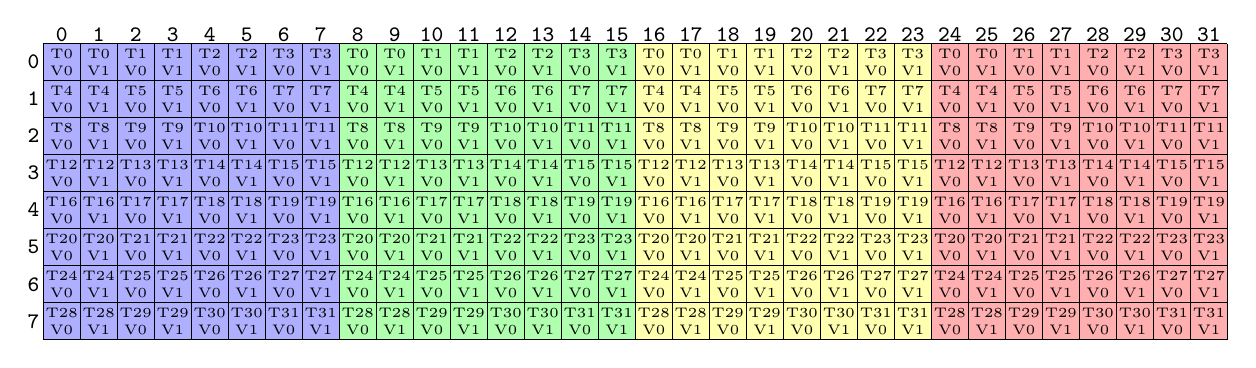
\begin{tikzpicture}[x={(0cm,-0.47cm)},y={(0.47cm,0cm)},every node/.style={minimum size=0.47cm, outer sep=0pt, inner sep=0pt, font=\tiny}]
\node[fill={rgb,255:red,175;green,175;blue,255}] at (0,0) {\shortstack{T0\\V0}};
\node[fill={rgb,255:red,175;green,175;blue,255}] at (0,1) {\shortstack{T0\\V1}};
\node[fill={rgb,255:red,175;green,175;blue,255}] at (0,2) {\shortstack{T1\\V0}};
\node[fill={rgb,255:red,175;green,175;blue,255}] at (0,3) {\shortstack{T1\\V1}};
\node[fill={rgb,255:red,175;green,175;blue,255}] at (0,4) {\shortstack{T2\\V0}};
\node[fill={rgb,255:red,175;green,175;blue,255}] at (0,5) {\shortstack{T2\\V1}};
\node[fill={rgb,255:red,175;green,175;blue,255}] at (0,6) {\shortstack{T3\\V0}};
\node[fill={rgb,255:red,175;green,175;blue,255}] at (0,7) {\shortstack{T3\\V1}};
\node[fill={rgb,255:red,175;green,255;blue,175}] at (0,8) {\shortstack{T0\\V0}};
\node[fill={rgb,255:red,175;green,255;blue,175}] at (0,9) {\shortstack{T0\\V1}};
\node[fill={rgb,255:red,175;green,255;blue,175}] at (0,10) {\shortstack{T1\\V0}};
\node[fill={rgb,255:red,175;green,255;blue,175}] at (0,11) {\shortstack{T1\\V1}};
\node[fill={rgb,255:red,175;green,255;blue,175}] at (0,12) {\shortstack{T2\\V0}};
\node[fill={rgb,255:red,175;green,255;blue,175}] at (0,13) {\shortstack{T2\\V1}};
\node[fill={rgb,255:red,175;green,255;blue,175}] at (0,14) {\shortstack{T3\\V0}};
\node[fill={rgb,255:red,175;green,255;blue,175}] at (0,15) {\shortstack{T3\\V1}};
\node[fill={rgb,255:red,255;green,255;blue,175}] at (0,16) {\shortstack{T0\\V0}};
\node[fill={rgb,255:red,255;green,255;blue,175}] at (0,17) {\shortstack{T0\\V1}};
\node[fill={rgb,255:red,255;green,255;blue,175}] at (0,18) {\shortstack{T1\\V0}};
\node[fill={rgb,255:red,255;green,255;blue,175}] at (0,19) {\shortstack{T1\\V1}};
\node[fill={rgb,255:red,255;green,255;blue,175}] at (0,20) {\shortstack{T2\\V0}};
\node[fill={rgb,255:red,255;green,255;blue,175}] at (0,21) {\shortstack{T2\\V1}};
\node[fill={rgb,255:red,255;green,255;blue,175}] at (0,22) {\shortstack{T3\\V0}};
\node[fill={rgb,255:red,255;green,255;blue,175}] at (0,23) {\shortstack{T3\\V1}};
\node[fill={rgb,255:red,255;green,175;blue,175}] at (0,24) {\shortstack{T0\\V0}};
\node[fill={rgb,255:red,255;green,175;blue,175}] at (0,25) {\shortstack{T0\\V1}};
\node[fill={rgb,255:red,255;green,175;blue,175}] at (0,26) {\shortstack{T1\\V0}};
\node[fill={rgb,255:red,255;green,175;blue,175}] at (0,27) {\shortstack{T1\\V1}};
\node[fill={rgb,255:red,255;green,175;blue,175}] at (0,28) {\shortstack{T2\\V0}};
\node[fill={rgb,255:red,255;green,175;blue,175}] at (0,29) {\shortstack{T2\\V1}};
\node[fill={rgb,255:red,255;green,175;blue,175}] at (0,30) {\shortstack{T3\\V0}};
\node[fill={rgb,255:red,255;green,175;blue,175}] at (0,31) {\shortstack{T3\\V1}};
\node[fill={rgb,255:red,175;green,175;blue,255}] at (1,0) {\shortstack{T4\\V0}};
\node[fill={rgb,255:red,175;green,175;blue,255}] at (1,1) {\shortstack{T4\\V1}};
\node[fill={rgb,255:red,175;green,175;blue,255}] at (1,2) {\shortstack{T5\\V0}};
\node[fill={rgb,255:red,175;green,175;blue,255}] at (1,3) {\shortstack{T5\\V1}};
\node[fill={rgb,255:red,175;green,175;blue,255}] at (1,4) {\shortstack{T6\\V0}};
\node[fill={rgb,255:red,175;green,175;blue,255}] at (1,5) {\shortstack{T6\\V1}};
\node[fill={rgb,255:red,175;green,175;blue,255}] at (1,6) {\shortstack{T7\\V0}};
\node[fill={rgb,255:red,175;green,175;blue,255}] at (1,7) {\shortstack{T7\\V1}};
\node[fill={rgb,255:red,175;green,255;blue,175}] at (1,8) {\shortstack{T4\\V0}};
\node[fill={rgb,255:red,175;green,255;blue,175}] at (1,9) {\shortstack{T4\\V1}};
\node[fill={rgb,255:red,175;green,255;blue,175}] at (1,10) {\shortstack{T5\\V0}};
\node[fill={rgb,255:red,175;green,255;blue,175}] at (1,11) {\shortstack{T5\\V1}};
\node[fill={rgb,255:red,175;green,255;blue,175}] at (1,12) {\shortstack{T6\\V0}};
\node[fill={rgb,255:red,175;green,255;blue,175}] at (1,13) {\shortstack{T6\\V1}};
\node[fill={rgb,255:red,175;green,255;blue,175}] at (1,14) {\shortstack{T7\\V0}};
\node[fill={rgb,255:red,175;green,255;blue,175}] at (1,15) {\shortstack{T7\\V1}};
\node[fill={rgb,255:red,255;green,255;blue,175}] at (1,16) {\shortstack{T4\\V0}};
\node[fill={rgb,255:red,255;green,255;blue,175}] at (1,17) {\shortstack{T4\\V1}};
\node[fill={rgb,255:red,255;green,255;blue,175}] at (1,18) {\shortstack{T5\\V0}};
\node[fill={rgb,255:red,255;green,255;blue,175}] at (1,19) {\shortstack{T5\\V1}};
\node[fill={rgb,255:red,255;green,255;blue,175}] at (1,20) {\shortstack{T6\\V0}};
\node[fill={rgb,255:red,255;green,255;blue,175}] at (1,21) {\shortstack{T6\\V1}};
\node[fill={rgb,255:red,255;green,255;blue,175}] at (1,22) {\shortstack{T7\\V0}};
\node[fill={rgb,255:red,255;green,255;blue,175}] at (1,23) {\shortstack{T7\\V1}};
\node[fill={rgb,255:red,255;green,175;blue,175}] at (1,24) {\shortstack{T4\\V0}};
\node[fill={rgb,255:red,255;green,175;blue,175}] at (1,25) {\shortstack{T4\\V1}};
\node[fill={rgb,255:red,255;green,175;blue,175}] at (1,26) {\shortstack{T5\\V0}};
\node[fill={rgb,255:red,255;green,175;blue,175}] at (1,27) {\shortstack{T5\\V1}};
\node[fill={rgb,255:red,255;green,175;blue,175}] at (1,28) {\shortstack{T6\\V0}};
\node[fill={rgb,255:red,255;green,175;blue,175}] at (1,29) {\shortstack{T6\\V1}};
\node[fill={rgb,255:red,255;green,175;blue,175}] at (1,30) {\shortstack{T7\\V0}};
\node[fill={rgb,255:red,255;green,175;blue,175}] at (1,31) {\shortstack{T7\\V1}};
\node[fill={rgb,255:red,175;green,175;blue,255}] at (2,0) {\shortstack{T8\\V0}};
\node[fill={rgb,255:red,175;green,175;blue,255}] at (2,1) {\shortstack{T8\\V1}};
\node[fill={rgb,255:red,175;green,175;blue,255}] at (2,2) {\shortstack{T9\\V0}};
\node[fill={rgb,255:red,175;green,175;blue,255}] at (2,3) {\shortstack{T9\\V1}};
\node[fill={rgb,255:red,175;green,175;blue,255}] at (2,4) {\shortstack{T10\\V0}};
\node[fill={rgb,255:red,175;green,175;blue,255}] at (2,5) {\shortstack{T10\\V1}};
\node[fill={rgb,255:red,175;green,175;blue,255}] at (2,6) {\shortstack{T11\\V0}};
\node[fill={rgb,255:red,175;green,175;blue,255}] at (2,7) {\shortstack{T11\\V1}};
\node[fill={rgb,255:red,175;green,255;blue,175}] at (2,8) {\shortstack{T8\\V0}};
\node[fill={rgb,255:red,175;green,255;blue,175}] at (2,9) {\shortstack{T8\\V1}};
\node[fill={rgb,255:red,175;green,255;blue,175}] at (2,10) {\shortstack{T9\\V0}};
\node[fill={rgb,255:red,175;green,255;blue,175}] at (2,11) {\shortstack{T9\\V1}};
\node[fill={rgb,255:red,175;green,255;blue,175}] at (2,12) {\shortstack{T10\\V0}};
\node[fill={rgb,255:red,175;green,255;blue,175}] at (2,13) {\shortstack{T10\\V1}};
\node[fill={rgb,255:red,175;green,255;blue,175}] at (2,14) {\shortstack{T11\\V0}};
\node[fill={rgb,255:red,175;green,255;blue,175}] at (2,15) {\shortstack{T11\\V1}};
\node[fill={rgb,255:red,255;green,255;blue,175}] at (2,16) {\shortstack{T8\\V0}};
\node[fill={rgb,255:red,255;green,255;blue,175}] at (2,17) {\shortstack{T8\\V1}};
\node[fill={rgb,255:red,255;green,255;blue,175}] at (2,18) {\shortstack{T9\\V0}};
\node[fill={rgb,255:red,255;green,255;blue,175}] at (2,19) {\shortstack{T9\\V1}};
\node[fill={rgb,255:red,255;green,255;blue,175}] at (2,20) {\shortstack{T10\\V0}};
\node[fill={rgb,255:red,255;green,255;blue,175}] at (2,21) {\shortstack{T10\\V1}};
\node[fill={rgb,255:red,255;green,255;blue,175}] at (2,22) {\shortstack{T11\\V0}};
\node[fill={rgb,255:red,255;green,255;blue,175}] at (2,23) {\shortstack{T11\\V1}};
\node[fill={rgb,255:red,255;green,175;blue,175}] at (2,24) {\shortstack{T8\\V0}};
\node[fill={rgb,255:red,255;green,175;blue,175}] at (2,25) {\shortstack{T8\\V1}};
\node[fill={rgb,255:red,255;green,175;blue,175}] at (2,26) {\shortstack{T9\\V0}};
\node[fill={rgb,255:red,255;green,175;blue,175}] at (2,27) {\shortstack{T9\\V1}};
\node[fill={rgb,255:red,255;green,175;blue,175}] at (2,28) {\shortstack{T10\\V0}};
\node[fill={rgb,255:red,255;green,175;blue,175}] at (2,29) {\shortstack{T10\\V1}};
\node[fill={rgb,255:red,255;green,175;blue,175}] at (2,30) {\shortstack{T11\\V0}};
\node[fill={rgb,255:red,255;green,175;blue,175}] at (2,31) {\shortstack{T11\\V1}};
\node[fill={rgb,255:red,175;green,175;blue,255}] at (3,0) {\shortstack{T12\\V0}};
\node[fill={rgb,255:red,175;green,175;blue,255}] at (3,1) {\shortstack{T12\\V1}};
\node[fill={rgb,255:red,175;green,175;blue,255}] at (3,2) {\shortstack{T13\\V0}};
\node[fill={rgb,255:red,175;green,175;blue,255}] at (3,3) {\shortstack{T13\\V1}};
\node[fill={rgb,255:red,175;green,175;blue,255}] at (3,4) {\shortstack{T14\\V0}};
\node[fill={rgb,255:red,175;green,175;blue,255}] at (3,5) {\shortstack{T14\\V1}};
\node[fill={rgb,255:red,175;green,175;blue,255}] at (3,6) {\shortstack{T15\\V0}};
\node[fill={rgb,255:red,175;green,175;blue,255}] at (3,7) {\shortstack{T15\\V1}};
\node[fill={rgb,255:red,175;green,255;blue,175}] at (3,8) {\shortstack{T12\\V0}};
\node[fill={rgb,255:red,175;green,255;blue,175}] at (3,9) {\shortstack{T12\\V1}};
\node[fill={rgb,255:red,175;green,255;blue,175}] at (3,10) {\shortstack{T13\\V0}};
\node[fill={rgb,255:red,175;green,255;blue,175}] at (3,11) {\shortstack{T13\\V1}};
\node[fill={rgb,255:red,175;green,255;blue,175}] at (3,12) {\shortstack{T14\\V0}};
\node[fill={rgb,255:red,175;green,255;blue,175}] at (3,13) {\shortstack{T14\\V1}};
\node[fill={rgb,255:red,175;green,255;blue,175}] at (3,14) {\shortstack{T15\\V0}};
\node[fill={rgb,255:red,175;green,255;blue,175}] at (3,15) {\shortstack{T15\\V1}};
\node[fill={rgb,255:red,255;green,255;blue,175}] at (3,16) {\shortstack{T12\\V0}};
\node[fill={rgb,255:red,255;green,255;blue,175}] at (3,17) {\shortstack{T12\\V1}};
\node[fill={rgb,255:red,255;green,255;blue,175}] at (3,18) {\shortstack{T13\\V0}};
\node[fill={rgb,255:red,255;green,255;blue,175}] at (3,19) {\shortstack{T13\\V1}};
\node[fill={rgb,255:red,255;green,255;blue,175}] at (3,20) {\shortstack{T14\\V0}};
\node[fill={rgb,255:red,255;green,255;blue,175}] at (3,21) {\shortstack{T14\\V1}};
\node[fill={rgb,255:red,255;green,255;blue,175}] at (3,22) {\shortstack{T15\\V0}};
\node[fill={rgb,255:red,255;green,255;blue,175}] at (3,23) {\shortstack{T15\\V1}};
\node[fill={rgb,255:red,255;green,175;blue,175}] at (3,24) {\shortstack{T12\\V0}};
\node[fill={rgb,255:red,255;green,175;blue,175}] at (3,25) {\shortstack{T12\\V1}};
\node[fill={rgb,255:red,255;green,175;blue,175}] at (3,26) {\shortstack{T13\\V0}};
\node[fill={rgb,255:red,255;green,175;blue,175}] at (3,27) {\shortstack{T13\\V1}};
\node[fill={rgb,255:red,255;green,175;blue,175}] at (3,28) {\shortstack{T14\\V0}};
\node[fill={rgb,255:red,255;green,175;blue,175}] at (3,29) {\shortstack{T14\\V1}};
\node[fill={rgb,255:red,255;green,175;blue,175}] at (3,30) {\shortstack{T15\\V0}};
\node[fill={rgb,255:red,255;green,175;blue,175}] at (3,31) {\shortstack{T15\\V1}};
\node[fill={rgb,255:red,175;green,175;blue,255}] at (4,0) {\shortstack{T16\\V0}};
\node[fill={rgb,255:red,175;green,175;blue,255}] at (4,1) {\shortstack{T16\\V1}};
\node[fill={rgb,255:red,175;green,175;blue,255}] at (4,2) {\shortstack{T17\\V0}};
\node[fill={rgb,255:red,175;green,175;blue,255}] at (4,3) {\shortstack{T17\\V1}};
\node[fill={rgb,255:red,175;green,175;blue,255}] at (4,4) {\shortstack{T18\\V0}};
\node[fill={rgb,255:red,175;green,175;blue,255}] at (4,5) {\shortstack{T18\\V1}};
\node[fill={rgb,255:red,175;green,175;blue,255}] at (4,6) {\shortstack{T19\\V0}};
\node[fill={rgb,255:red,175;green,175;blue,255}] at (4,7) {\shortstack{T19\\V1}};
\node[fill={rgb,255:red,175;green,255;blue,175}] at (4,8) {\shortstack{T16\\V0}};
\node[fill={rgb,255:red,175;green,255;blue,175}] at (4,9) {\shortstack{T16\\V1}};
\node[fill={rgb,255:red,175;green,255;blue,175}] at (4,10) {\shortstack{T17\\V0}};
\node[fill={rgb,255:red,175;green,255;blue,175}] at (4,11) {\shortstack{T17\\V1}};
\node[fill={rgb,255:red,175;green,255;blue,175}] at (4,12) {\shortstack{T18\\V0}};
\node[fill={rgb,255:red,175;green,255;blue,175}] at (4,13) {\shortstack{T18\\V1}};
\node[fill={rgb,255:red,175;green,255;blue,175}] at (4,14) {\shortstack{T19\\V0}};
\node[fill={rgb,255:red,175;green,255;blue,175}] at (4,15) {\shortstack{T19\\V1}};
\node[fill={rgb,255:red,255;green,255;blue,175}] at (4,16) {\shortstack{T16\\V0}};
\node[fill={rgb,255:red,255;green,255;blue,175}] at (4,17) {\shortstack{T16\\V1}};
\node[fill={rgb,255:red,255;green,255;blue,175}] at (4,18) {\shortstack{T17\\V0}};
\node[fill={rgb,255:red,255;green,255;blue,175}] at (4,19) {\shortstack{T17\\V1}};
\node[fill={rgb,255:red,255;green,255;blue,175}] at (4,20) {\shortstack{T18\\V0}};
\node[fill={rgb,255:red,255;green,255;blue,175}] at (4,21) {\shortstack{T18\\V1}};
\node[fill={rgb,255:red,255;green,255;blue,175}] at (4,22) {\shortstack{T19\\V0}};
\node[fill={rgb,255:red,255;green,255;blue,175}] at (4,23) {\shortstack{T19\\V1}};
\node[fill={rgb,255:red,255;green,175;blue,175}] at (4,24) {\shortstack{T16\\V0}};
\node[fill={rgb,255:red,255;green,175;blue,175}] at (4,25) {\shortstack{T16\\V1}};
\node[fill={rgb,255:red,255;green,175;blue,175}] at (4,26) {\shortstack{T17\\V0}};
\node[fill={rgb,255:red,255;green,175;blue,175}] at (4,27) {\shortstack{T17\\V1}};
\node[fill={rgb,255:red,255;green,175;blue,175}] at (4,28) {\shortstack{T18\\V0}};
\node[fill={rgb,255:red,255;green,175;blue,175}] at (4,29) {\shortstack{T18\\V1}};
\node[fill={rgb,255:red,255;green,175;blue,175}] at (4,30) {\shortstack{T19\\V0}};
\node[fill={rgb,255:red,255;green,175;blue,175}] at (4,31) {\shortstack{T19\\V1}};
\node[fill={rgb,255:red,175;green,175;blue,255}] at (5,0) {\shortstack{T20\\V0}};
\node[fill={rgb,255:red,175;green,175;blue,255}] at (5,1) {\shortstack{T20\\V1}};
\node[fill={rgb,255:red,175;green,175;blue,255}] at (5,2) {\shortstack{T21\\V0}};
\node[fill={rgb,255:red,175;green,175;blue,255}] at (5,3) {\shortstack{T21\\V1}};
\node[fill={rgb,255:red,175;green,175;blue,255}] at (5,4) {\shortstack{T22\\V0}};
\node[fill={rgb,255:red,175;green,175;blue,255}] at (5,5) {\shortstack{T22\\V1}};
\node[fill={rgb,255:red,175;green,175;blue,255}] at (5,6) {\shortstack{T23\\V0}};
\node[fill={rgb,255:red,175;green,175;blue,255}] at (5,7) {\shortstack{T23\\V1}};
\node[fill={rgb,255:red,175;green,255;blue,175}] at (5,8) {\shortstack{T20\\V0}};
\node[fill={rgb,255:red,175;green,255;blue,175}] at (5,9) {\shortstack{T20\\V1}};
\node[fill={rgb,255:red,175;green,255;blue,175}] at (5,10) {\shortstack{T21\\V0}};
\node[fill={rgb,255:red,175;green,255;blue,175}] at (5,11) {\shortstack{T21\\V1}};
\node[fill={rgb,255:red,175;green,255;blue,175}] at (5,12) {\shortstack{T22\\V0}};
\node[fill={rgb,255:red,175;green,255;blue,175}] at (5,13) {\shortstack{T22\\V1}};
\node[fill={rgb,255:red,175;green,255;blue,175}] at (5,14) {\shortstack{T23\\V0}};
\node[fill={rgb,255:red,175;green,255;blue,175}] at (5,15) {\shortstack{T23\\V1}};
\node[fill={rgb,255:red,255;green,255;blue,175}] at (5,16) {\shortstack{T20\\V0}};
\node[fill={rgb,255:red,255;green,255;blue,175}] at (5,17) {\shortstack{T20\\V1}};
\node[fill={rgb,255:red,255;green,255;blue,175}] at (5,18) {\shortstack{T21\\V0}};
\node[fill={rgb,255:red,255;green,255;blue,175}] at (5,19) {\shortstack{T21\\V1}};
\node[fill={rgb,255:red,255;green,255;blue,175}] at (5,20) {\shortstack{T22\\V0}};
\node[fill={rgb,255:red,255;green,255;blue,175}] at (5,21) {\shortstack{T22\\V1}};
\node[fill={rgb,255:red,255;green,255;blue,175}] at (5,22) {\shortstack{T23\\V0}};
\node[fill={rgb,255:red,255;green,255;blue,175}] at (5,23) {\shortstack{T23\\V1}};
\node[fill={rgb,255:red,255;green,175;blue,175}] at (5,24) {\shortstack{T20\\V0}};
\node[fill={rgb,255:red,255;green,175;blue,175}] at (5,25) {\shortstack{T20\\V1}};
\node[fill={rgb,255:red,255;green,175;blue,175}] at (5,26) {\shortstack{T21\\V0}};
\node[fill={rgb,255:red,255;green,175;blue,175}] at (5,27) {\shortstack{T21\\V1}};
\node[fill={rgb,255:red,255;green,175;blue,175}] at (5,28) {\shortstack{T22\\V0}};
\node[fill={rgb,255:red,255;green,175;blue,175}] at (5,29) {\shortstack{T22\\V1}};
\node[fill={rgb,255:red,255;green,175;blue,175}] at (5,30) {\shortstack{T23\\V0}};
\node[fill={rgb,255:red,255;green,175;blue,175}] at (5,31) {\shortstack{T23\\V1}};
\node[fill={rgb,255:red,175;green,175;blue,255}] at (6,0) {\shortstack{T24\\V0}};
\node[fill={rgb,255:red,175;green,175;blue,255}] at (6,1) {\shortstack{T24\\V1}};
\node[fill={rgb,255:red,175;green,175;blue,255}] at (6,2) {\shortstack{T25\\V0}};
\node[fill={rgb,255:red,175;green,175;blue,255}] at (6,3) {\shortstack{T25\\V1}};
\node[fill={rgb,255:red,175;green,175;blue,255}] at (6,4) {\shortstack{T26\\V0}};
\node[fill={rgb,255:red,175;green,175;blue,255}] at (6,5) {\shortstack{T26\\V1}};
\node[fill={rgb,255:red,175;green,175;blue,255}] at (6,6) {\shortstack{T27\\V0}};
\node[fill={rgb,255:red,175;green,175;blue,255}] at (6,7) {\shortstack{T27\\V1}};
\node[fill={rgb,255:red,175;green,255;blue,175}] at (6,8) {\shortstack{T24\\V0}};
\node[fill={rgb,255:red,175;green,255;blue,175}] at (6,9) {\shortstack{T24\\V1}};
\node[fill={rgb,255:red,175;green,255;blue,175}] at (6,10) {\shortstack{T25\\V0}};
\node[fill={rgb,255:red,175;green,255;blue,175}] at (6,11) {\shortstack{T25\\V1}};
\node[fill={rgb,255:red,175;green,255;blue,175}] at (6,12) {\shortstack{T26\\V0}};
\node[fill={rgb,255:red,175;green,255;blue,175}] at (6,13) {\shortstack{T26\\V1}};
\node[fill={rgb,255:red,175;green,255;blue,175}] at (6,14) {\shortstack{T27\\V0}};
\node[fill={rgb,255:red,175;green,255;blue,175}] at (6,15) {\shortstack{T27\\V1}};
\node[fill={rgb,255:red,255;green,255;blue,175}] at (6,16) {\shortstack{T24\\V0}};
\node[fill={rgb,255:red,255;green,255;blue,175}] at (6,17) {\shortstack{T24\\V1}};
\node[fill={rgb,255:red,255;green,255;blue,175}] at (6,18) {\shortstack{T25\\V0}};
\node[fill={rgb,255:red,255;green,255;blue,175}] at (6,19) {\shortstack{T25\\V1}};
\node[fill={rgb,255:red,255;green,255;blue,175}] at (6,20) {\shortstack{T26\\V0}};
\node[fill={rgb,255:red,255;green,255;blue,175}] at (6,21) {\shortstack{T26\\V1}};
\node[fill={rgb,255:red,255;green,255;blue,175}] at (6,22) {\shortstack{T27\\V0}};
\node[fill={rgb,255:red,255;green,255;blue,175}] at (6,23) {\shortstack{T27\\V1}};
\node[fill={rgb,255:red,255;green,175;blue,175}] at (6,24) {\shortstack{T24\\V0}};
\node[fill={rgb,255:red,255;green,175;blue,175}] at (6,25) {\shortstack{T24\\V1}};
\node[fill={rgb,255:red,255;green,175;blue,175}] at (6,26) {\shortstack{T25\\V0}};
\node[fill={rgb,255:red,255;green,175;blue,175}] at (6,27) {\shortstack{T25\\V1}};
\node[fill={rgb,255:red,255;green,175;blue,175}] at (6,28) {\shortstack{T26\\V0}};
\node[fill={rgb,255:red,255;green,175;blue,175}] at (6,29) {\shortstack{T26\\V1}};
\node[fill={rgb,255:red,255;green,175;blue,175}] at (6,30) {\shortstack{T27\\V0}};
\node[fill={rgb,255:red,255;green,175;blue,175}] at (6,31) {\shortstack{T27\\V1}};
\node[fill={rgb,255:red,175;green,175;blue,255}] at (7,0) {\shortstack{T28\\V0}};
\node[fill={rgb,255:red,175;green,175;blue,255}] at (7,1) {\shortstack{T28\\V1}};
\node[fill={rgb,255:red,175;green,175;blue,255}] at (7,2) {\shortstack{T29\\V0}};
\node[fill={rgb,255:red,175;green,175;blue,255}] at (7,3) {\shortstack{T29\\V1}};
\node[fill={rgb,255:red,175;green,175;blue,255}] at (7,4) {\shortstack{T30\\V0}};
\node[fill={rgb,255:red,175;green,175;blue,255}] at (7,5) {\shortstack{T30\\V1}};
\node[fill={rgb,255:red,175;green,175;blue,255}] at (7,6) {\shortstack{T31\\V0}};
\node[fill={rgb,255:red,175;green,175;blue,255}] at (7,7) {\shortstack{T31\\V1}};
\node[fill={rgb,255:red,175;green,255;blue,175}] at (7,8) {\shortstack{T28\\V0}};
\node[fill={rgb,255:red,175;green,255;blue,175}] at (7,9) {\shortstack{T28\\V1}};
\node[fill={rgb,255:red,175;green,255;blue,175}] at (7,10) {\shortstack{T29\\V0}};
\node[fill={rgb,255:red,175;green,255;blue,175}] at (7,11) {\shortstack{T29\\V1}};
\node[fill={rgb,255:red,175;green,255;blue,175}] at (7,12) {\shortstack{T30\\V0}};
\node[fill={rgb,255:red,175;green,255;blue,175}] at (7,13) {\shortstack{T30\\V1}};
\node[fill={rgb,255:red,175;green,255;blue,175}] at (7,14) {\shortstack{T31\\V0}};
\node[fill={rgb,255:red,175;green,255;blue,175}] at (7,15) {\shortstack{T31\\V1}};
\node[fill={rgb,255:red,255;green,255;blue,175}] at (7,16) {\shortstack{T28\\V0}};
\node[fill={rgb,255:red,255;green,255;blue,175}] at (7,17) {\shortstack{T28\\V1}};
\node[fill={rgb,255:red,255;green,255;blue,175}] at (7,18) {\shortstack{T29\\V0}};
\node[fill={rgb,255:red,255;green,255;blue,175}] at (7,19) {\shortstack{T29\\V1}};
\node[fill={rgb,255:red,255;green,255;blue,175}] at (7,20) {\shortstack{T30\\V0}};
\node[fill={rgb,255:red,255;green,255;blue,175}] at (7,21) {\shortstack{T30\\V1}};
\node[fill={rgb,255:red,255;green,255;blue,175}] at (7,22) {\shortstack{T31\\V0}};
\node[fill={rgb,255:red,255;green,255;blue,175}] at (7,23) {\shortstack{T31\\V1}};
\node[fill={rgb,255:red,255;green,175;blue,175}] at (7,24) {\shortstack{T28\\V0}};
\node[fill={rgb,255:red,255;green,175;blue,175}] at (7,25) {\shortstack{T28\\V1}};
\node[fill={rgb,255:red,255;green,175;blue,175}] at (7,26) {\shortstack{T29\\V0}};
\node[fill={rgb,255:red,255;green,175;blue,175}] at (7,27) {\shortstack{T29\\V1}};
\node[fill={rgb,255:red,255;green,175;blue,175}] at (7,28) {\shortstack{T30\\V0}};
\node[fill={rgb,255:red,255;green,175;blue,175}] at (7,29) {\shortstack{T30\\V1}};
\node[fill={rgb,255:red,255;green,175;blue,175}] at (7,30) {\shortstack{T31\\V0}};
\node[fill={rgb,255:red,255;green,175;blue,175}] at (7,31) {\shortstack{T31\\V1}};
\draw[color=black,thin,step=0.47cm,shift={(-0.5,-0.5)}] (0,0) grid (8,32);
\node[anchor=east,minimum size=0pt,font=\footnotesize] at (0,-0.6) {\texttt{0}};
\node[anchor=east,minimum size=0pt,font=\footnotesize] at (1,-0.6) {\texttt{1}};
\node[anchor=east,minimum size=0pt,font=\footnotesize] at (2,-0.6) {\texttt{2}};
\node[anchor=east,minimum size=0pt,font=\footnotesize] at (3,-0.6) {\texttt{3}};
\node[anchor=east,minimum size=0pt,font=\footnotesize] at (4,-0.6) {\texttt{4}};
\node[anchor=east,minimum size=0pt,font=\footnotesize] at (5,-0.6) {\texttt{5}};
\node[anchor=east,minimum size=0pt,font=\footnotesize] at (6,-0.6) {\texttt{6}};
\node[anchor=east,minimum size=0pt,font=\footnotesize] at (7,-0.6) {\texttt{7}};
\node[minimum size=0pt,font=\footnotesize] at (-0.75,0) {\texttt{0}};
\node[minimum size=0pt,font=\footnotesize] at (-0.75,1) {\texttt{1}};
\node[minimum size=0pt,font=\footnotesize] at (-0.75,2) {\texttt{2}};
\node[minimum size=0pt,font=\footnotesize] at (-0.75,3) {\texttt{3}};
\node[minimum size=0pt,font=\footnotesize] at (-0.75,4) {\texttt{4}};
\node[minimum size=0pt,font=\footnotesize] at (-0.75,5) {\texttt{5}};
\node[minimum size=0pt,font=\footnotesize] at (-0.75,6) {\texttt{6}};
\node[minimum size=0pt,font=\footnotesize] at (-0.75,7) {\texttt{7}};
\node[minimum size=0pt,font=\footnotesize] at (-0.75,8) {\texttt{8}};
\node[minimum size=0pt,font=\footnotesize] at (-0.75,9) {\texttt{9}};
\node[minimum size=0pt,font=\footnotesize] at (-0.75,10) {\texttt{10}};
\node[minimum size=0pt,font=\footnotesize] at (-0.75,11) {\texttt{11}};
\node[minimum size=0pt,font=\footnotesize] at (-0.75,12) {\texttt{12}};
\node[minimum size=0pt,font=\footnotesize] at (-0.75,13) {\texttt{13}};
\node[minimum size=0pt,font=\footnotesize] at (-0.75,14) {\texttt{14}};
\node[minimum size=0pt,font=\footnotesize] at (-0.75,15) {\texttt{15}};
\node[minimum size=0pt,font=\footnotesize] at (-0.75,16) {\texttt{16}};
\node[minimum size=0pt,font=\footnotesize] at (-0.75,17) {\texttt{17}};
\node[minimum size=0pt,font=\footnotesize] at (-0.75,18) {\texttt{18}};
\node[minimum size=0pt,font=\footnotesize] at (-0.75,19) {\texttt{19}};
\node[minimum size=0pt,font=\footnotesize] at (-0.75,20) {\texttt{20}};
\node[minimum size=0pt,font=\footnotesize] at (-0.75,21) {\texttt{21}};
\node[minimum size=0pt,font=\footnotesize] at (-0.75,22) {\texttt{22}};
\node[minimum size=0pt,font=\footnotesize] at (-0.75,23) {\texttt{23}};
\node[minimum size=0pt,font=\footnotesize] at (-0.75,24) {\texttt{24}};
\node[minimum size=0pt,font=\footnotesize] at (-0.75,25) {\texttt{25}};
\node[minimum size=0pt,font=\footnotesize] at (-0.75,26) {\texttt{26}};
\node[minimum size=0pt,font=\footnotesize] at (-0.75,27) {\texttt{27}};
\node[minimum size=0pt,font=\footnotesize] at (-0.75,28) {\texttt{28}};
\node[minimum size=0pt,font=\footnotesize] at (-0.75,29) {\texttt{29}};
\node[minimum size=0pt,font=\footnotesize] at (-0.75,30) {\texttt{30}};
\node[minimum size=0pt,font=\footnotesize] at (-0.75,31) {\texttt{31}};
\end{tikzpicture}
\end{center}

Both are dense bijections, as Definition~\ref{def:validity} requires of a map
into $\logical$. Composed onto storage they become address maps, and
Section~\ref{sec:decide} emits their code. With the $16 \times 16$ tile
stored row-major with leading dimension $24$, that is with
$(16,16){:}(24,1) : \logical \to \physical$ in place of
$\mathrm{canonical}((16,16))$, the two-warp map is decided to be a layout and
the emitted address is
\begin{center}
\verb|8*c0 + 24*c1_0_0 + 2*c1_0_1 + 192*c1_1_0 + c1_1_1|
\end{center}
where \verb|c0| is the warp and \verb|c1_0_0|, \verb|c1_0_1|,
\verb|c1_1_0|, \verb|c1_1_1| are $g$, $t_4$, $v_m$, $v_n$: the address
$24(g + 8v_m) + 8w + 2t_4 + v_n$. The slice for warp $1$
(Section~\ref{sec:restrict}) is
\begin{center}
\verb|24*c1_0_0 + 2*c1_0_1 + 192*c1_1_0 + c1_1_1 + 8|
\end{center}
With the $8 \times 32$ tile stored with leading dimension $40$, the
\texttt{ldmatrix} map emits
\begin{center}
\verb|8*c0 + 40*c1_0_0 + 2*c1_0_1 + c1_1|
\end{center}
with \verb|c0| the matrix and \verb|c1_0_0|, \verb|c1_0_1|, \verb|c1_1|
the lane's $g$ and $q$ and the value $v$. The tests build the same
construction for a $32 \times 16$ tile and four warps, and the
\texttt{ldmatrix} reader of a GEMM mainloop (Section~\ref{sec:eval}).

\paragraph{Usage.} The table lists the idioms CUTLASS kernels are written
with and what each is in our algebra. $L|_{x = v}$ fixes the entries named
$x$ to $v$ (Definition~\ref{def:restrict}). $F : \tv \to \logical$ is a valid
map, such as $F_C$ above; $W$ is a dense bijection arranging the warps, as
above; and $T : \logical \to \tv$ is a dense bijection from the positions of
a tile to the threads.

\begin{center}\small
\begin{tabular}{@{}p{0.34\linewidth}p{0.62\linewidth}@{}}
\toprule
\textbf{CuTe} & \textbf{Our algebra} \\
\midrule
\texttt{make\_layout(S, D)} & $S{:}D$, modes reversed \\
\texttt{composition(A, B)} & $A \circ B$ \\
\texttt{complement(B, M)} & rest of $\divideop(\mathrm{canonical}(R), S)$, above \\
\texttt{logical\_divide(A, S)}, \texttt{zipped\_divide} & $\divideop(A, S)$ \\
\texttt{local\_tile(A, S, b)} & $\divideop(A,S)\big|_{\mathrm{rest} = b}$ \\
\texttt{local\_partition(A, T, t)} & $\divideop(A, S_T)\big|_{\mathrm{tile} = \mathrm{inverse}(T)(t)}$ \\
\texttt{partition\_A/B/C}, \texttt{tensor(\_, k)} & $(A \circ F)\big|_{\mathrm{thread} = t}$; $A\big|_{k}$ \\
\texttt{logical\_product(A, B)}, \texttt{blocked\_product}, \texttt{tile\_to\_shape} & $\repeatop(A, B)$, $A$ a dense bijection \\
\texttt{raked\_product(A, B)} & $\repeatop(A, B)$ with the two coordinate groups exchanged in each mode \\
\texttt{logical\_product(B, A)}, copies first & $\interleave(A, B)$, $B$ a dense bijection, up to the order of the groups \\
stride-$0$ modes & $\broadcast(L, S)$; read-only \\
\texttt{Swizzle<B,M,S>} $\circ\ L$ & $\sigma \circ L$ with $b = B$, $\mathit{dst} = M$, $\mathit{src} = M{+}S$ (Definition~\ref{def:swizzle}) \\
$k$-stage pipeline buffer & $\repeatop(L, k{:}1)$ \\
\texttt{TiledCopy}: \texttt{partition\_S/D}, vector width $v$ & $\divideop(A, (1,v)) \circ \interleave(v{:}1,\ 32{:}1)$ over the lanes \\
\texttt{TiledMMA}: $F$ over a CTA tile with warp grid $W$ & $\divideop(A, S_F) \circ \interleave(F, W)$ \\
\texttt{right\_inverse(L)}; \texttt{retile\_S/D} & $\mathrm{inverse}(L)$; $\mathrm{inverse}(F_{\mathrm{mma}}) \circ F_{\mathrm{copy}}$ \\
\texttt{coalesce} & not needed: the kernel declares the shape it iterates \\
\texttt{group\_modes}, \texttt{select}, \texttt{flatten} & regrouping the shape; same function \\
\texttt{recast}, \texttt{upcast} by $v$ & $\divideop(A, (1,\dots,1,v))$; the change of element size is outside the algebra \\
TMA box $S$; multicast & $\divideop(A, S)$; $\broadcast$ across CTAs \\
\bottomrule
\end{tabular}
\end{center}

Every row is one of composition, $\divideop$, $\restrict$, $\repeatop$,
$\interleave$, $\broadcast$, a swizzle, $\mathrm{inverse}$, or a regrouping of
a shape.

\section{Evaluation}\label{sec:eval}

The implementation\footnote{\url{https://github.com/annp0/simplified-layout}}
is 983 lines of OCaml; the tests are 2{,}305.
\claude{These line counts match no counting of the tree. The 2026-09-19 draft generates every number in this section from the test suite (\texttt{papers/eval.sh}); suggest re-adopting that.}

\paragraph{The decision procedure is correct.} The criterion of
Lemma~\ref{lem:dense} agrees with enumeration on 400 random layouts. The scan of
Theorem~\ref{thm:decide} is compared with an oracle that tries every chain of
divisors of $n$ and checks the strides it forces at every point. Over every
function $g : [0,n) \to [0,k)$ with $g(0) = 0$, for
$n \in \{2,3,4,6,8,9,12\}$ and $k = 5$ if $n \le 4$, $3$ otherwise, that is
186{,}293 functions, the two accept the same 58, with the same chain.

\paragraph{It matters in practice.} Of the 178 layouts the tests build from
CUTLASS's atoms and CuTe's examples, 147 are affine in their coordinates, 9
are layouts of a refinement with one coordinate split, and 22 are not layouts
and are emitted as composites. On 600 random composites of a dense bijection
with a padded storage map, 524 are layouts of some refinement, and their
emitted forms contain 686 divisions and moduli where the composites contain
1{,}026. With a random swizzle on the storage map, none of 300 is a layout.
\claude{Three numbers here disagree with the tests: 524 should be 531, 686 should be 646, and 1{,}026 should be 976 (the seeds are fixed; the prose was transcribed once and left behind). The 178/147/9/22 were right for An's tree but became 207/172/11/24 once two coverage gaps in the oracle were closed.}

\paragraph{The algebra is enough for a kernel.} The SM90 GMMA $64 \times
128$ accumulator, built from the SM80 \texttt{mma.m16n8k16} $C$ fragment as
\[
\divideop\big(\mathrm{canonical}((64,128)),\ (16,8)\big) \circ
\interleave\big(F_C,\ \mathrm{canonical}((4,16))\big),
\]
equals NVIDIA's printed layout at all 8192 coordinates. A GEMM mainloop
built from the operations alone, an $8 \times 32$ tile of 16-bit elements
copied in 16-byte vectors by one warp into two shared-memory stages of the
SW64 atom and read back by \texttt{ldmatrix}, with the writer and reader of
Section~\ref{sec:cute} and the stages by $\repeatop$, is consistent: for
every element, the address the copy writes is the address the \texttt{mma}
operand is read from.

\section{Related work}\label{sec:related}

\textbf{CuTe}~\cite{cutedocs,cecka} is the system under study; its operations
and their conditions are stated in Section~\ref{sec:intro}.
\textbf{Shah}~\cite{shah} formalizes the algebra and gives the conditions
under which the composite of two layouts is again a layout. In our algebra
that is decided after the fact by Theorem~\ref{thm:decide}, and a composite
that is not a layout is still a legal map. \textbf{Carlisle et
al.}~\cite{categorical} model a class of CuTe layouts as morphisms of two
categories, define composition, logical product and logical division on the
morphisms, and characterize the layouts so obtained. \textbf{Linear
layouts}~\cite{triton}, in Triton, represent a layout as a matrix over
$\mathbb{F}_2$ acting on the bits of the hardware index, which gives generic
layout-to-layout conversion; a swizzle of Definition~\ref{def:swizzle} is such
a matrix. \textbf{Bhaskaracharya et al.}~\cite{isl} represent both CuTe
layouts and linear layouts as integer set relations in ISL and implement
composition, inversion and complement with its operations; the question of
Section~\ref{sec:decide} can be posed there, and Theorem~\ref{thm:decide}
answers it without a solver. \textbf{Axe}~\cite{axe} maps logical
coordinates to a multi-axis physical space through named axes and unifies
tiling, sharding, replication and offsets from device meshes to threads; its
replication is explicit, as $\broadcast$ is in our algebra, and its
Appendix~A.2.1 uses the floor expansion and first differences of
Section~\ref{sec:decide} to prove a normalized representation unique.
\textbf{Halide}~\cite{halide}, \textbf{TVM}~\cite{tvm} and
\textbf{MLIR}~\cite{mlir} carry general integer expression simplifiers;
Section~\ref{sec:decide} decides the layout question directly instead.

\section{Conclusion}\label{sec:conclusion}

CuTe's layout algebra guards its operations with admissibility conditions
that its API does not show, and it may silently fail when one is violated.
We propose a new layout algebra in which each layout declares the space it
maps into, and that declaration alone reduces those conditions to one. The
algebra still reproduces CuTe's documented examples and CUTLASS's atoms, and
its decision procedure and operations are proved in Rocq.

The next step is to compile with these layouts: a GPU DSL in which each warp
is a SIMD program and warps communicate through pipes, so that kernels built
from the algebra alone can be measured against their CuTe counterparts.

\begin{thebibliography}{9}

\bibitem{cutedocs}
NVIDIA. \emph{CuTe: Layouts and Layout Algebra}. CUTLASS documentation,
\texttt{docs.nvidia.com/cutlass}, accessed 2026.

\bibitem{cecka}
C.~Cecka. \emph{CuTe Layout Representation and Algebra}. NVIDIA Research;
arXiv:2603.02298, 2026.

\bibitem{shah}
J.~Shah. \emph{A Note on the Algebra of CuTe Layouts}. Colfax Research
technical note, 2024.

\bibitem{categorical}
J.~Carlisle, J.~Shah, R.~Stern, P.~VanKoughnett.
\emph{Categorical Foundations for CuTe Layouts}. arXiv:2601.05972, 2026.

\bibitem{triton}
K.~Zhou, M.~Lezcano, A.~Goucher, A.~Rakhmati, J.~Niu, J.~Lebar, P.~Szczerbuk,
P.~Bell, P.~Tillet, T.~Raoux, Z.~Moudallal. \emph{Linear Layouts: Robust Code
Generation of Efficient Tensor Computation Using $\mathbb{F}_2$}. ASPLOS 2026;
arXiv:2505.23819.

\bibitem{isl}
S.~G.~Bhaskaracharya, A.~Acharya, B.~Hagedorn, V.~Grover. \emph{Modeling
Layout Abstractions Using Integer Set Relations}. arXiv:2511.10374, 2025.

\bibitem{axe}
B.~Hou, H.~Jin, G.~Wang, J.~Chen, Y.~Cai, L.~Yang, Z.~Ye, Y.~Ding, R.~Lai,
T.~Chen. \emph{Axe: A Simple Unified Layout Abstraction for Machine Learning
Compilers}. arXiv:2601.19092, 2026.

\bibitem{ptx}
NVIDIA. \emph{Parallel Thread Execution ISA}. Matrix fragment layout tables,
accessed 2026.

\bibitem{halide}
J.~Ragan-Kelley, C.~Barnes, A.~Adams, S.~Paris, F.~Durand, S.~Amarasinghe.
\emph{Halide: A Language and Compiler for Optimizing Parallelism, Locality,
and Recomputation in Image Processing Pipelines}. PLDI 2013.

\bibitem{tvm}
T.~Chen et al. \emph{TVM: An Automated End-to-End Optimizing Compiler for
Deep Learning}. OSDI 2018.

\bibitem{mlir}
C.~Lattner et al. \emph{MLIR: Scaling Compiler Infrastructure for Domain
Specific Computation}. CGO 2021.

\end{thebibliography}


\end{document}
